\documentclass[tikz,crop,convert={density=200,outext=.png},border=0.4cm]{standalone}

\usepackage{pgfplots}
\usepackage{amsmath}
\usetikzlibrary{arrows.meta}
\usepackage{physics}
\usepackage{xcolor}
% The exponential model
\definecolor{exp_1}{RGB}{0,68,27}
\definecolor{exp_2}{RGB}{35,139,69}
% The logistic model
\definecolor{log_1}{RGB}{8,64,129}
\definecolor{log_2}{RGB}{43,140,190}
% The logistic model
\definecolor{gen_1}{RGB}{127,0,0}
\definecolor{gen_2}{RGB}{215,48,31}
% General tikz settings for the axes etc.
\pgfplotsset{compat=newest,
    %width=6cm,
    %height=3cm,
    scale only axis=true,
    max space between ticks=25pt,
    try min ticks=5,
    every axis/.style={
        axis y line=left,
        axis x line=bottom,
        axis line style={thick,->,>=latex, shorten >=-.3cm}
    },
    every axis plot/.append style={thick},
    tick style={black, thick},
}
\tikzset{
    semithick/.style={line width=0.8pt},
}
\usepgfplotslibrary{groupplots}
\usepgfplotslibrary{dateplot}
% Document begins
\begin{document}
% =========================================================================================================
% t=0
\begin{tikzpicture}
\node[inner sep=0pt] (mixed) at (0,0)
{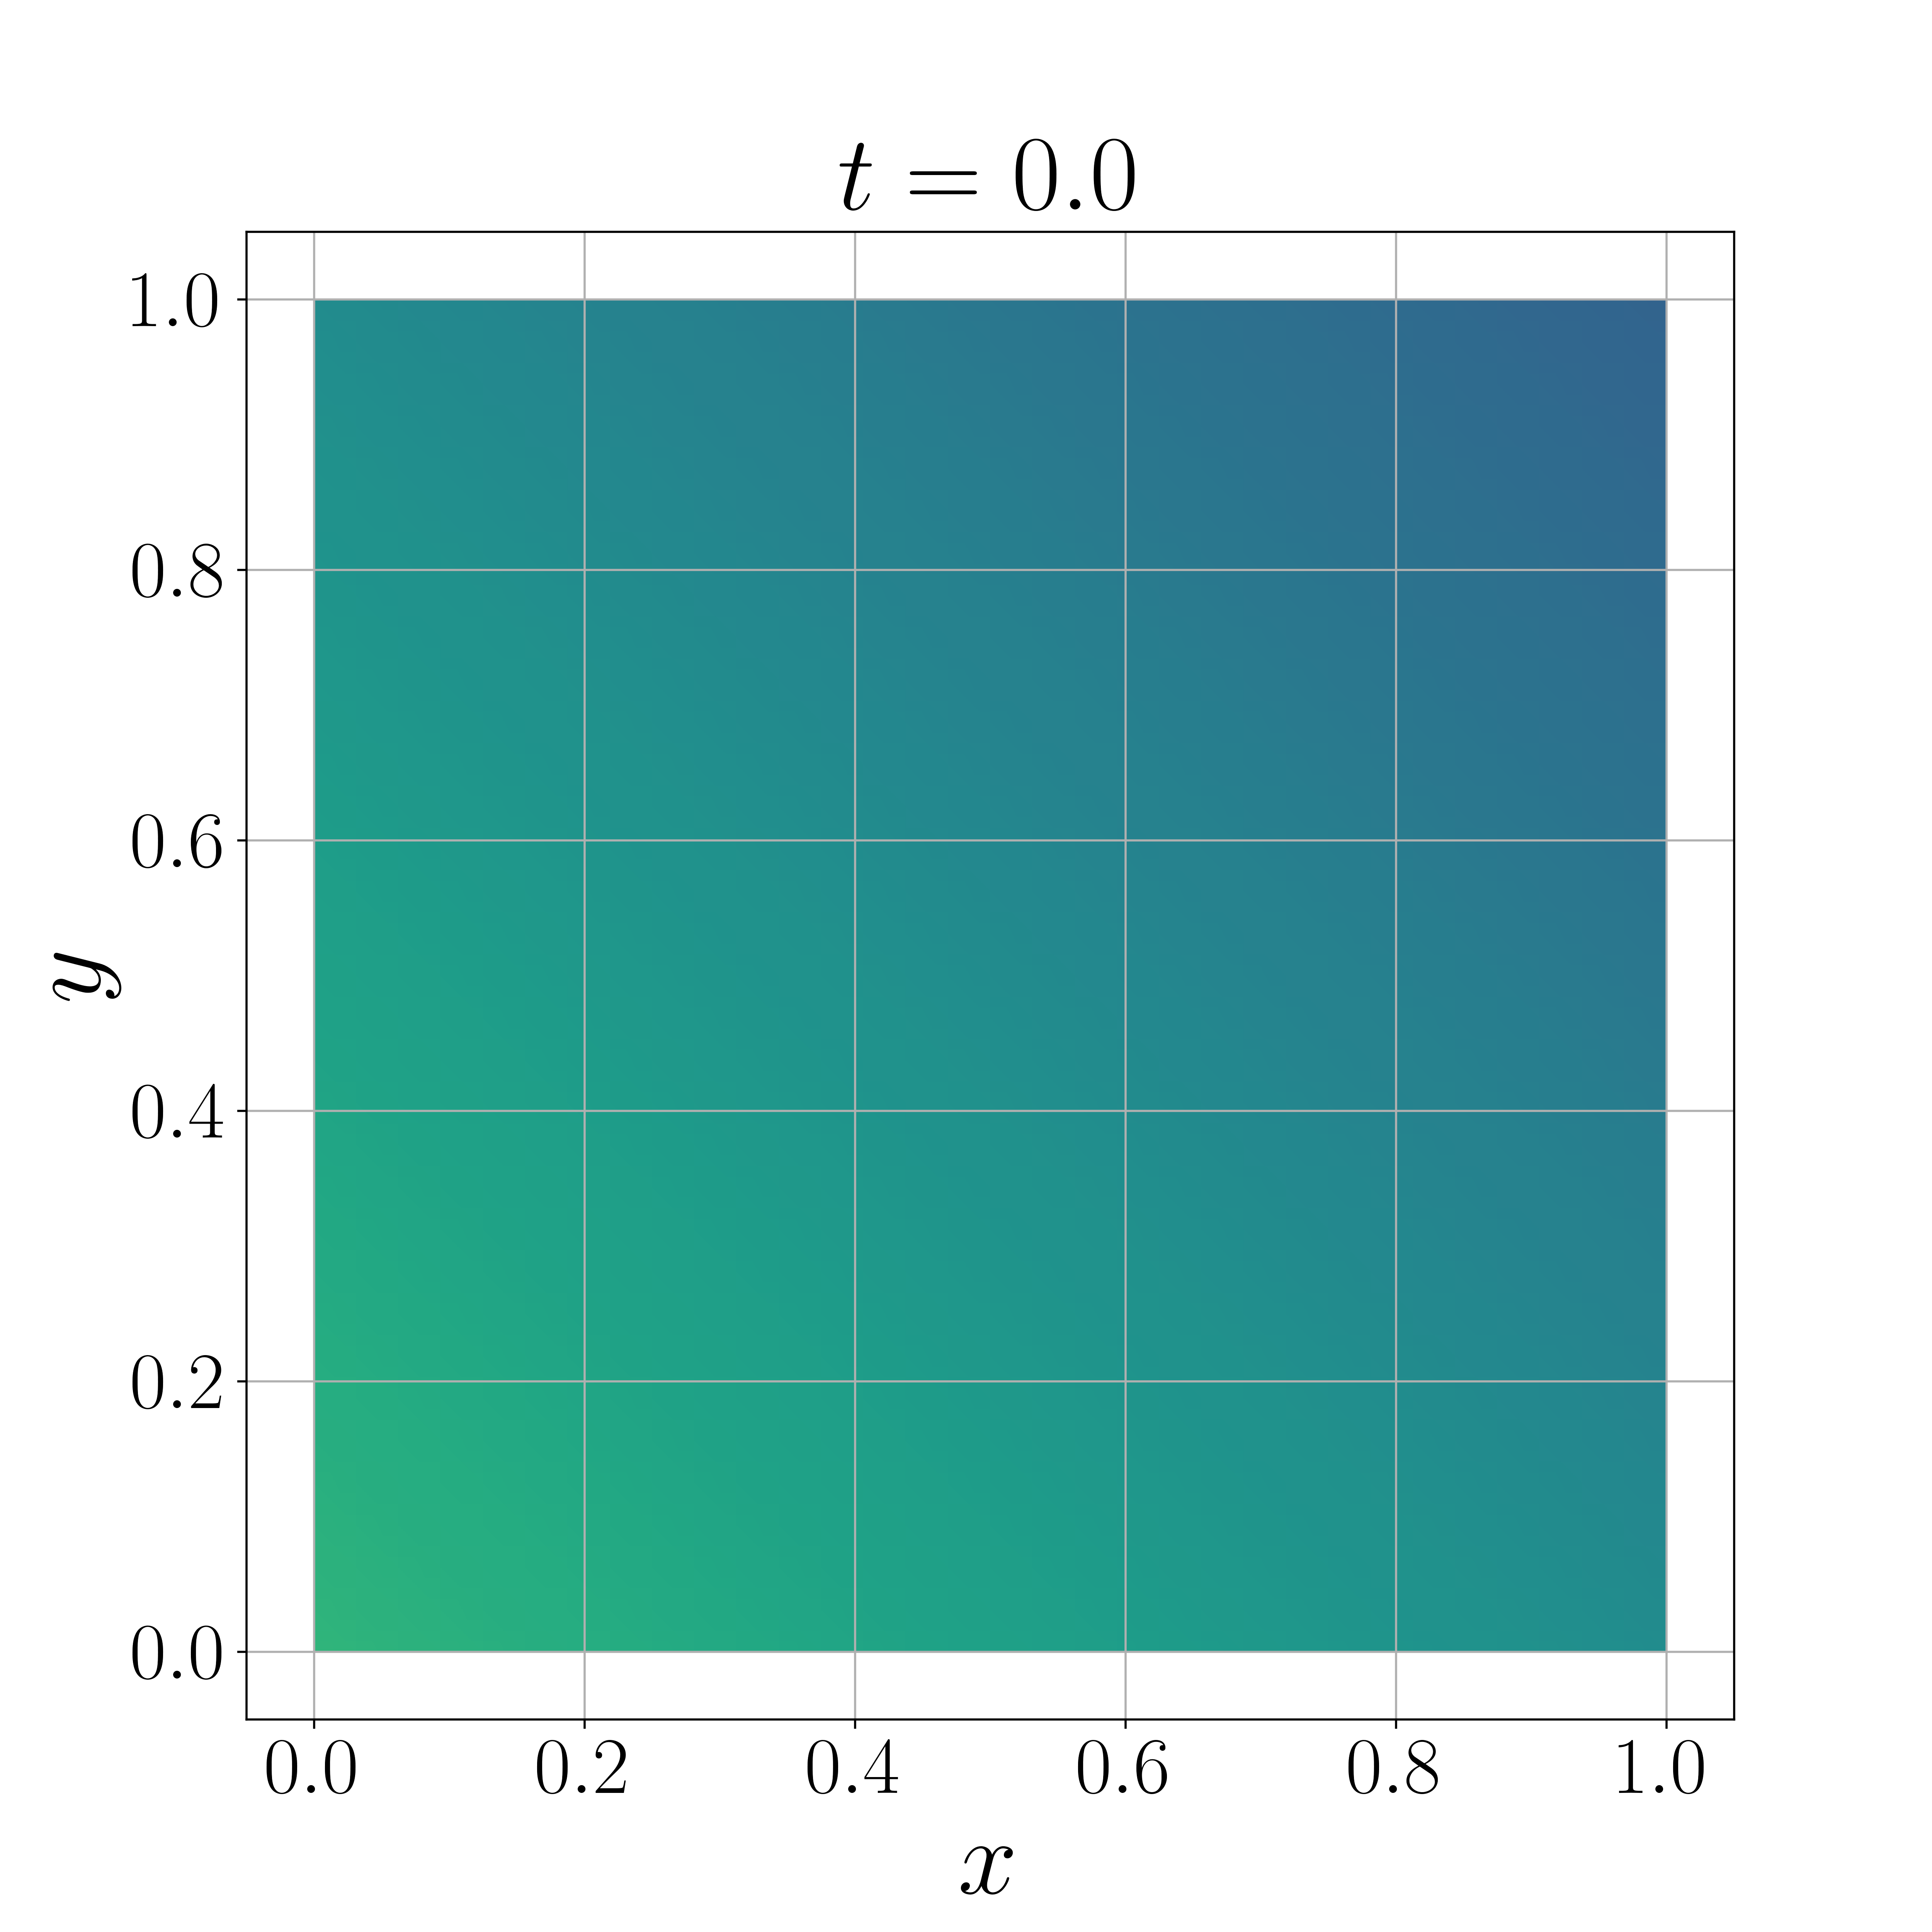
\includegraphics[width=\textwidth]{{./Input/cx_0p707_0p707_0p0}}};
\end{tikzpicture}
% =========================================================================================================
% =========================================================================================================
% t=0.2
\begin{tikzpicture}
\node[inner sep=0pt] (mixed) at (0,0)
{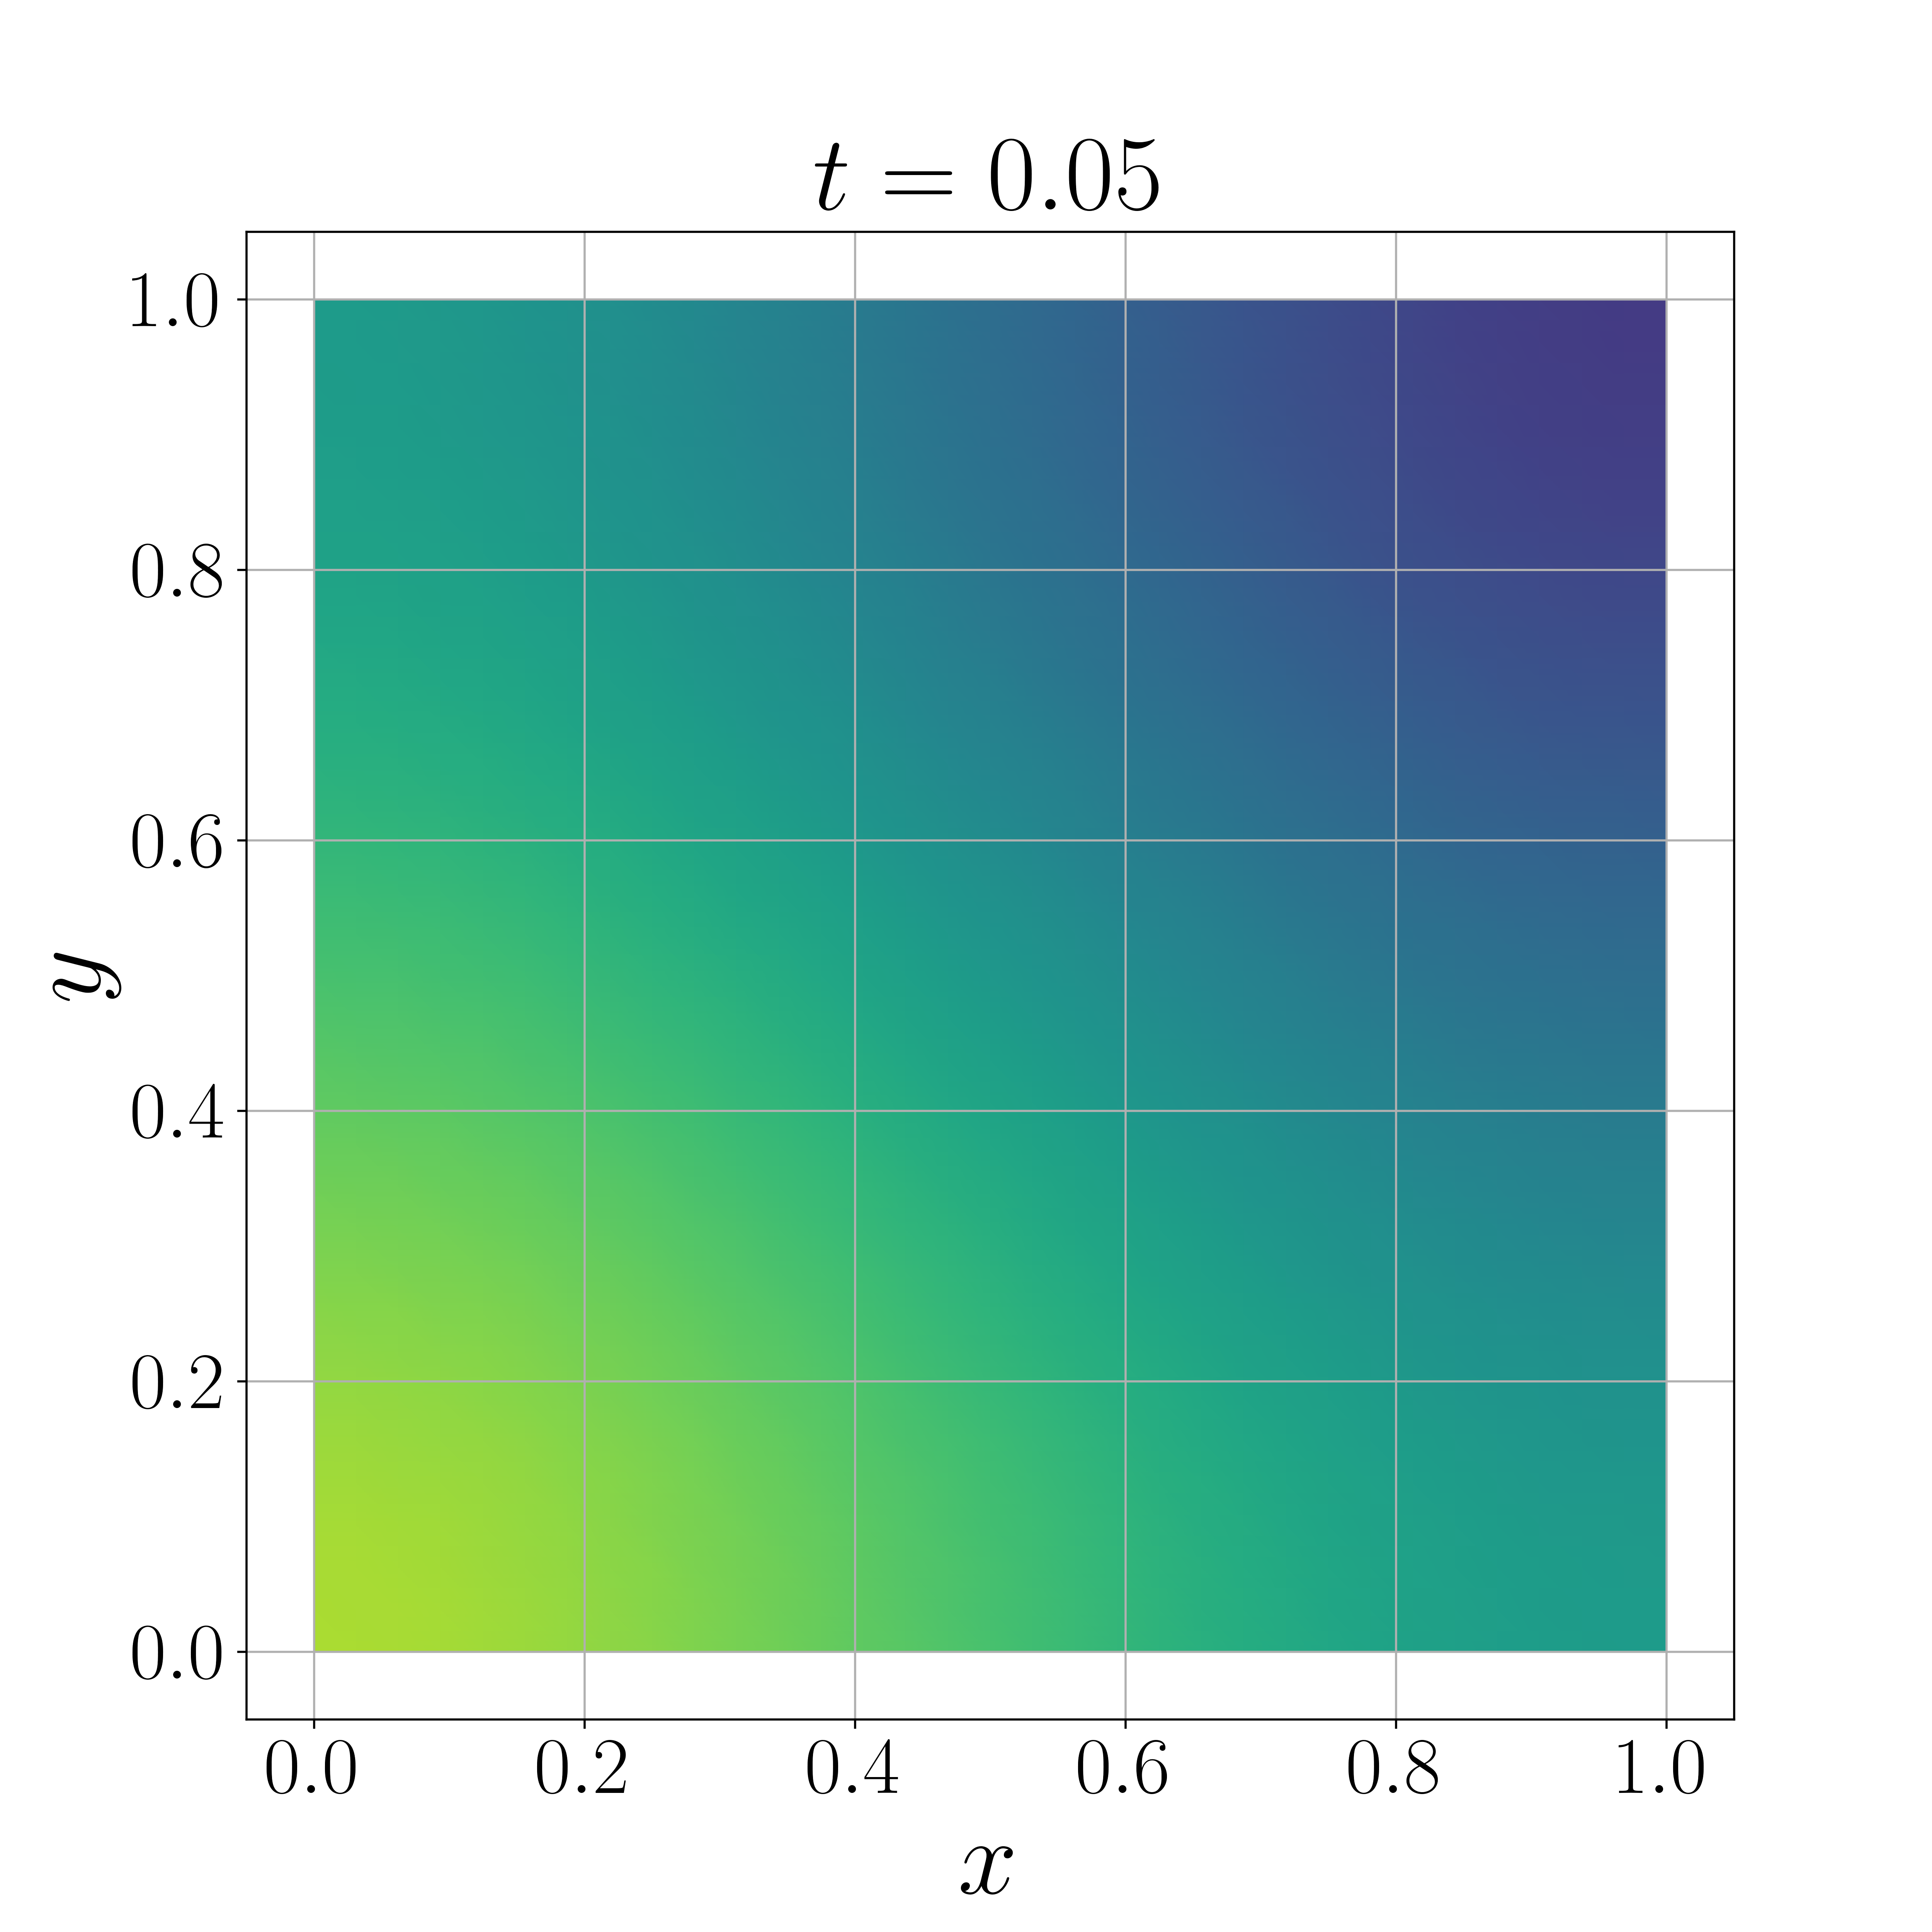
\includegraphics[width=\textwidth]{{./Input/cx_0p707_0p707_0p05}}};
\end{tikzpicture}
% =========================================================================================================
% =========================================================================================================
% t=0.3
\begin{tikzpicture}
\node[inner sep=0pt] (mixed) at (0,0)
{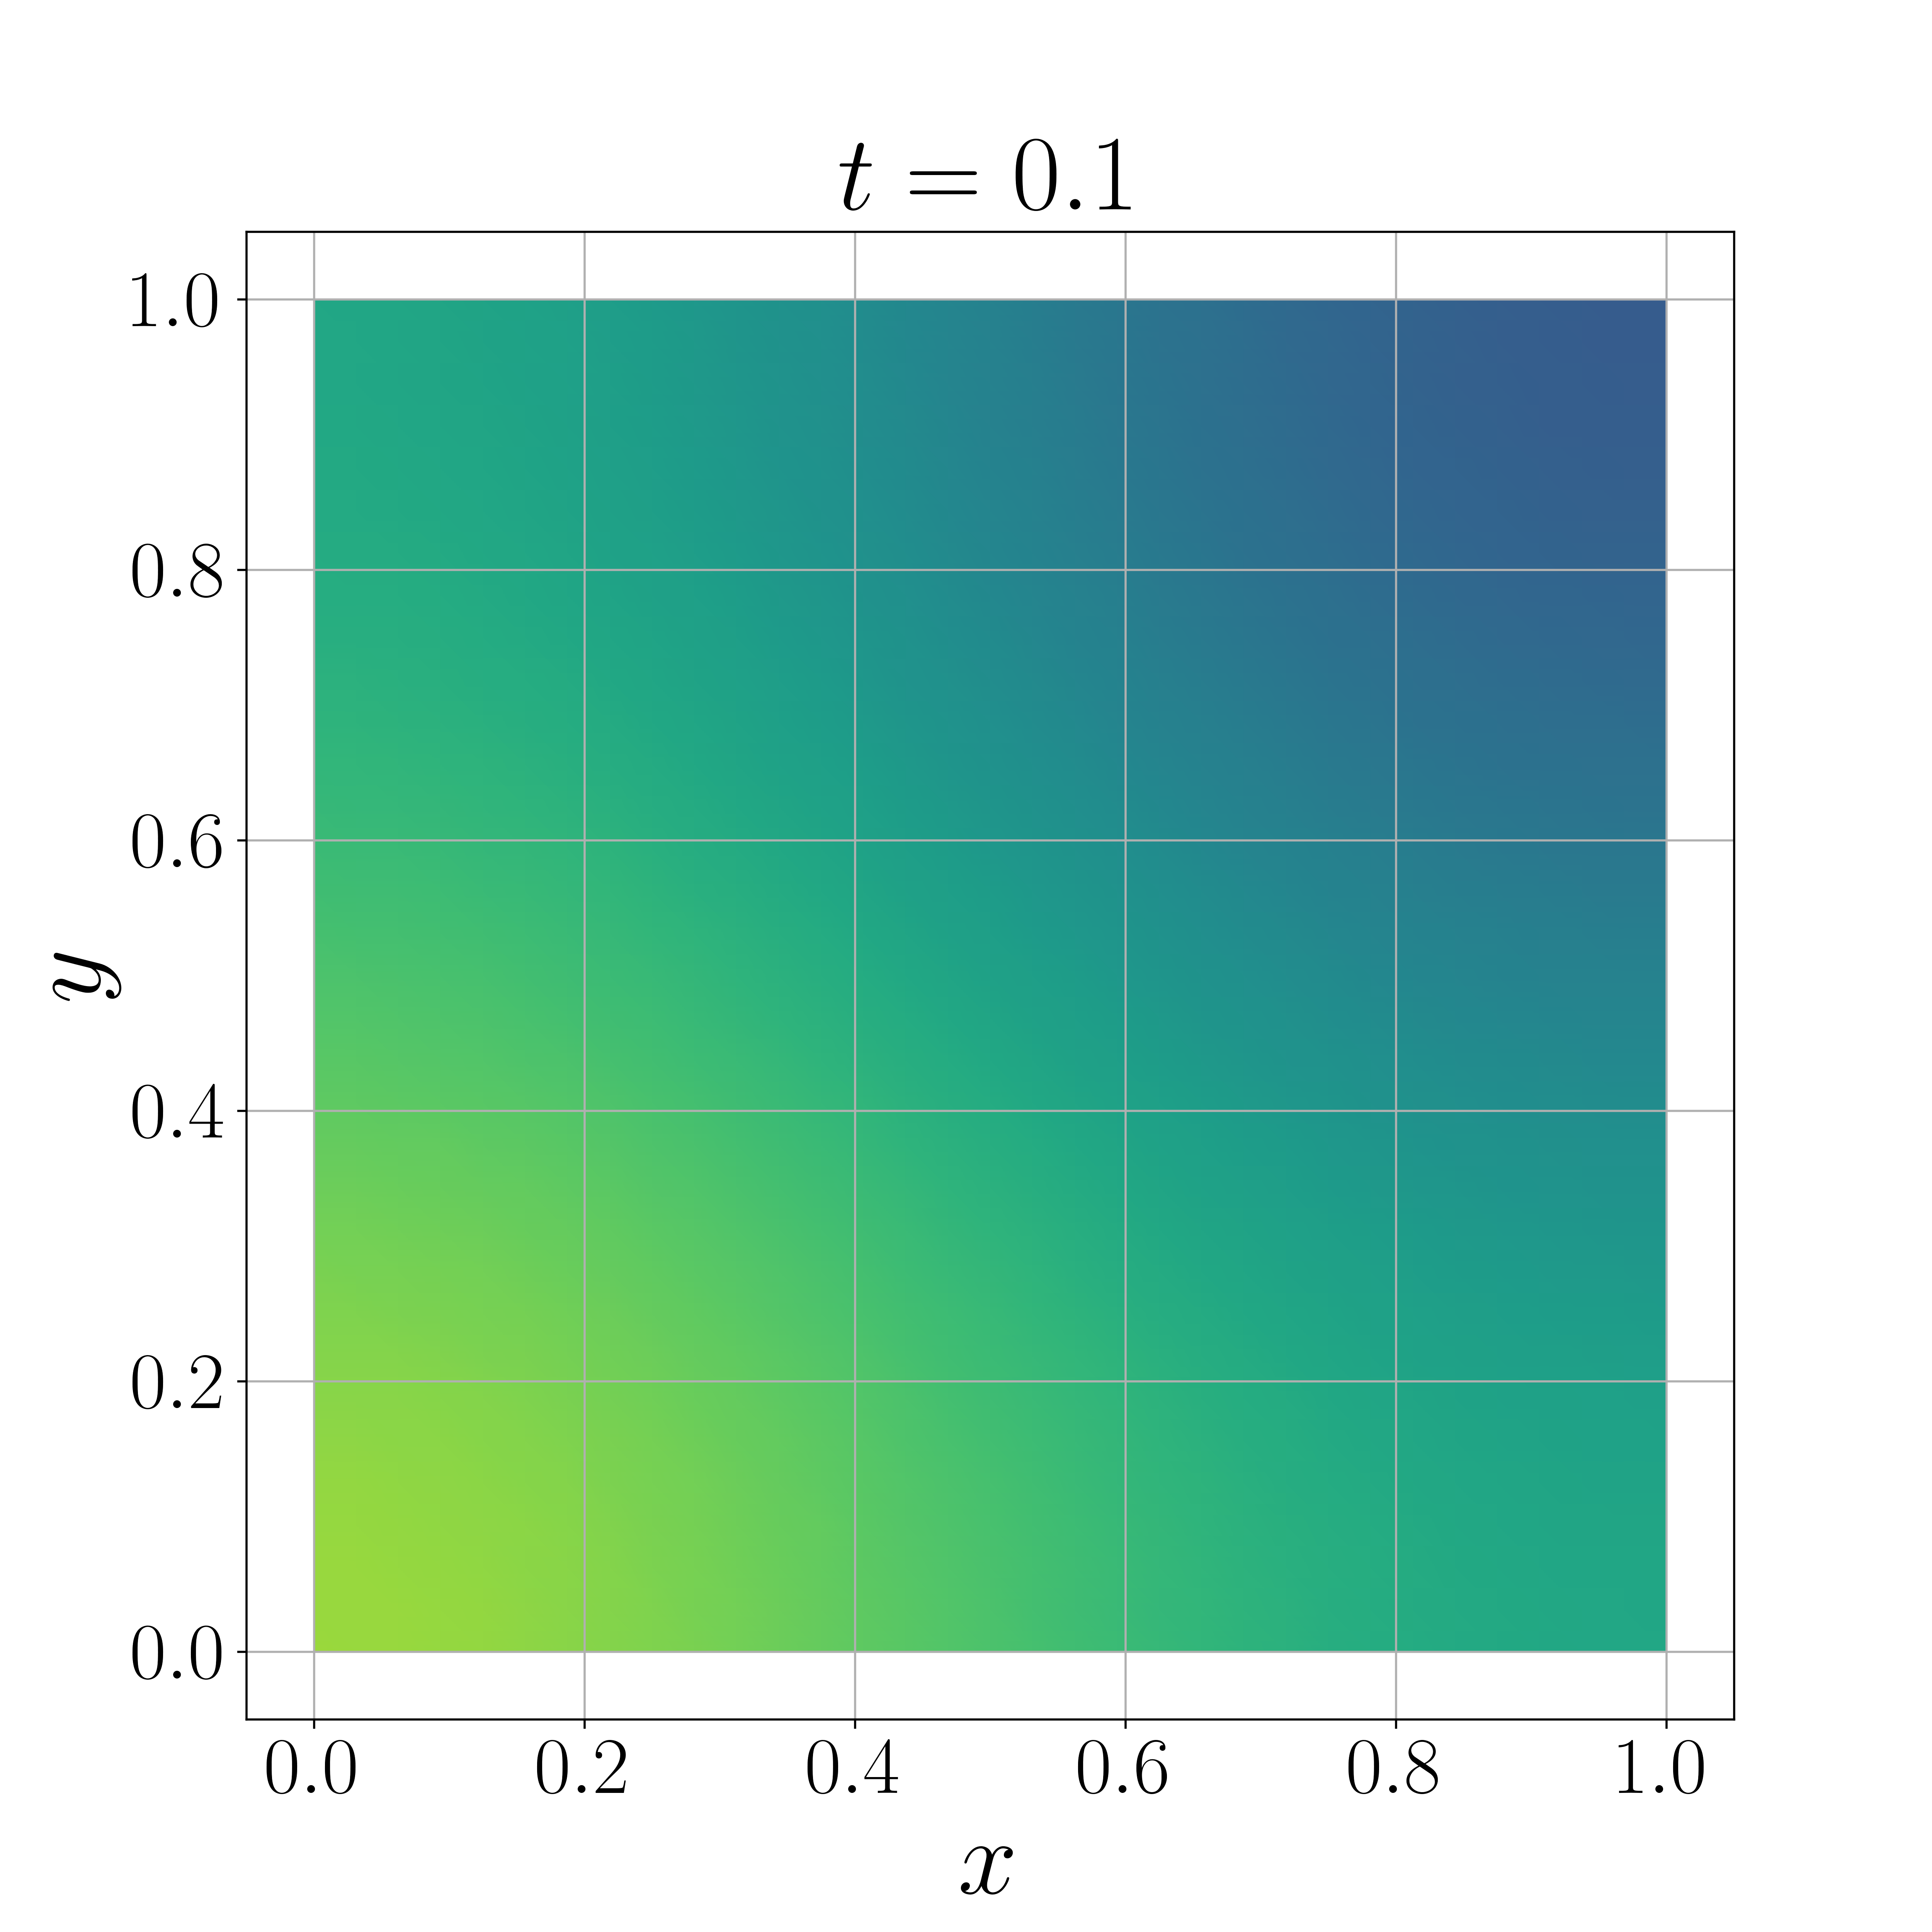
\includegraphics[width=\textwidth]{{./Input/cx_0p707_0p707_0p1}}};
\end{tikzpicture}
% =========================================================================================================
% =========================================================================================================
% t=0.4
\begin{tikzpicture}
\node[inner sep=0pt] (mixed) at (0,0)
{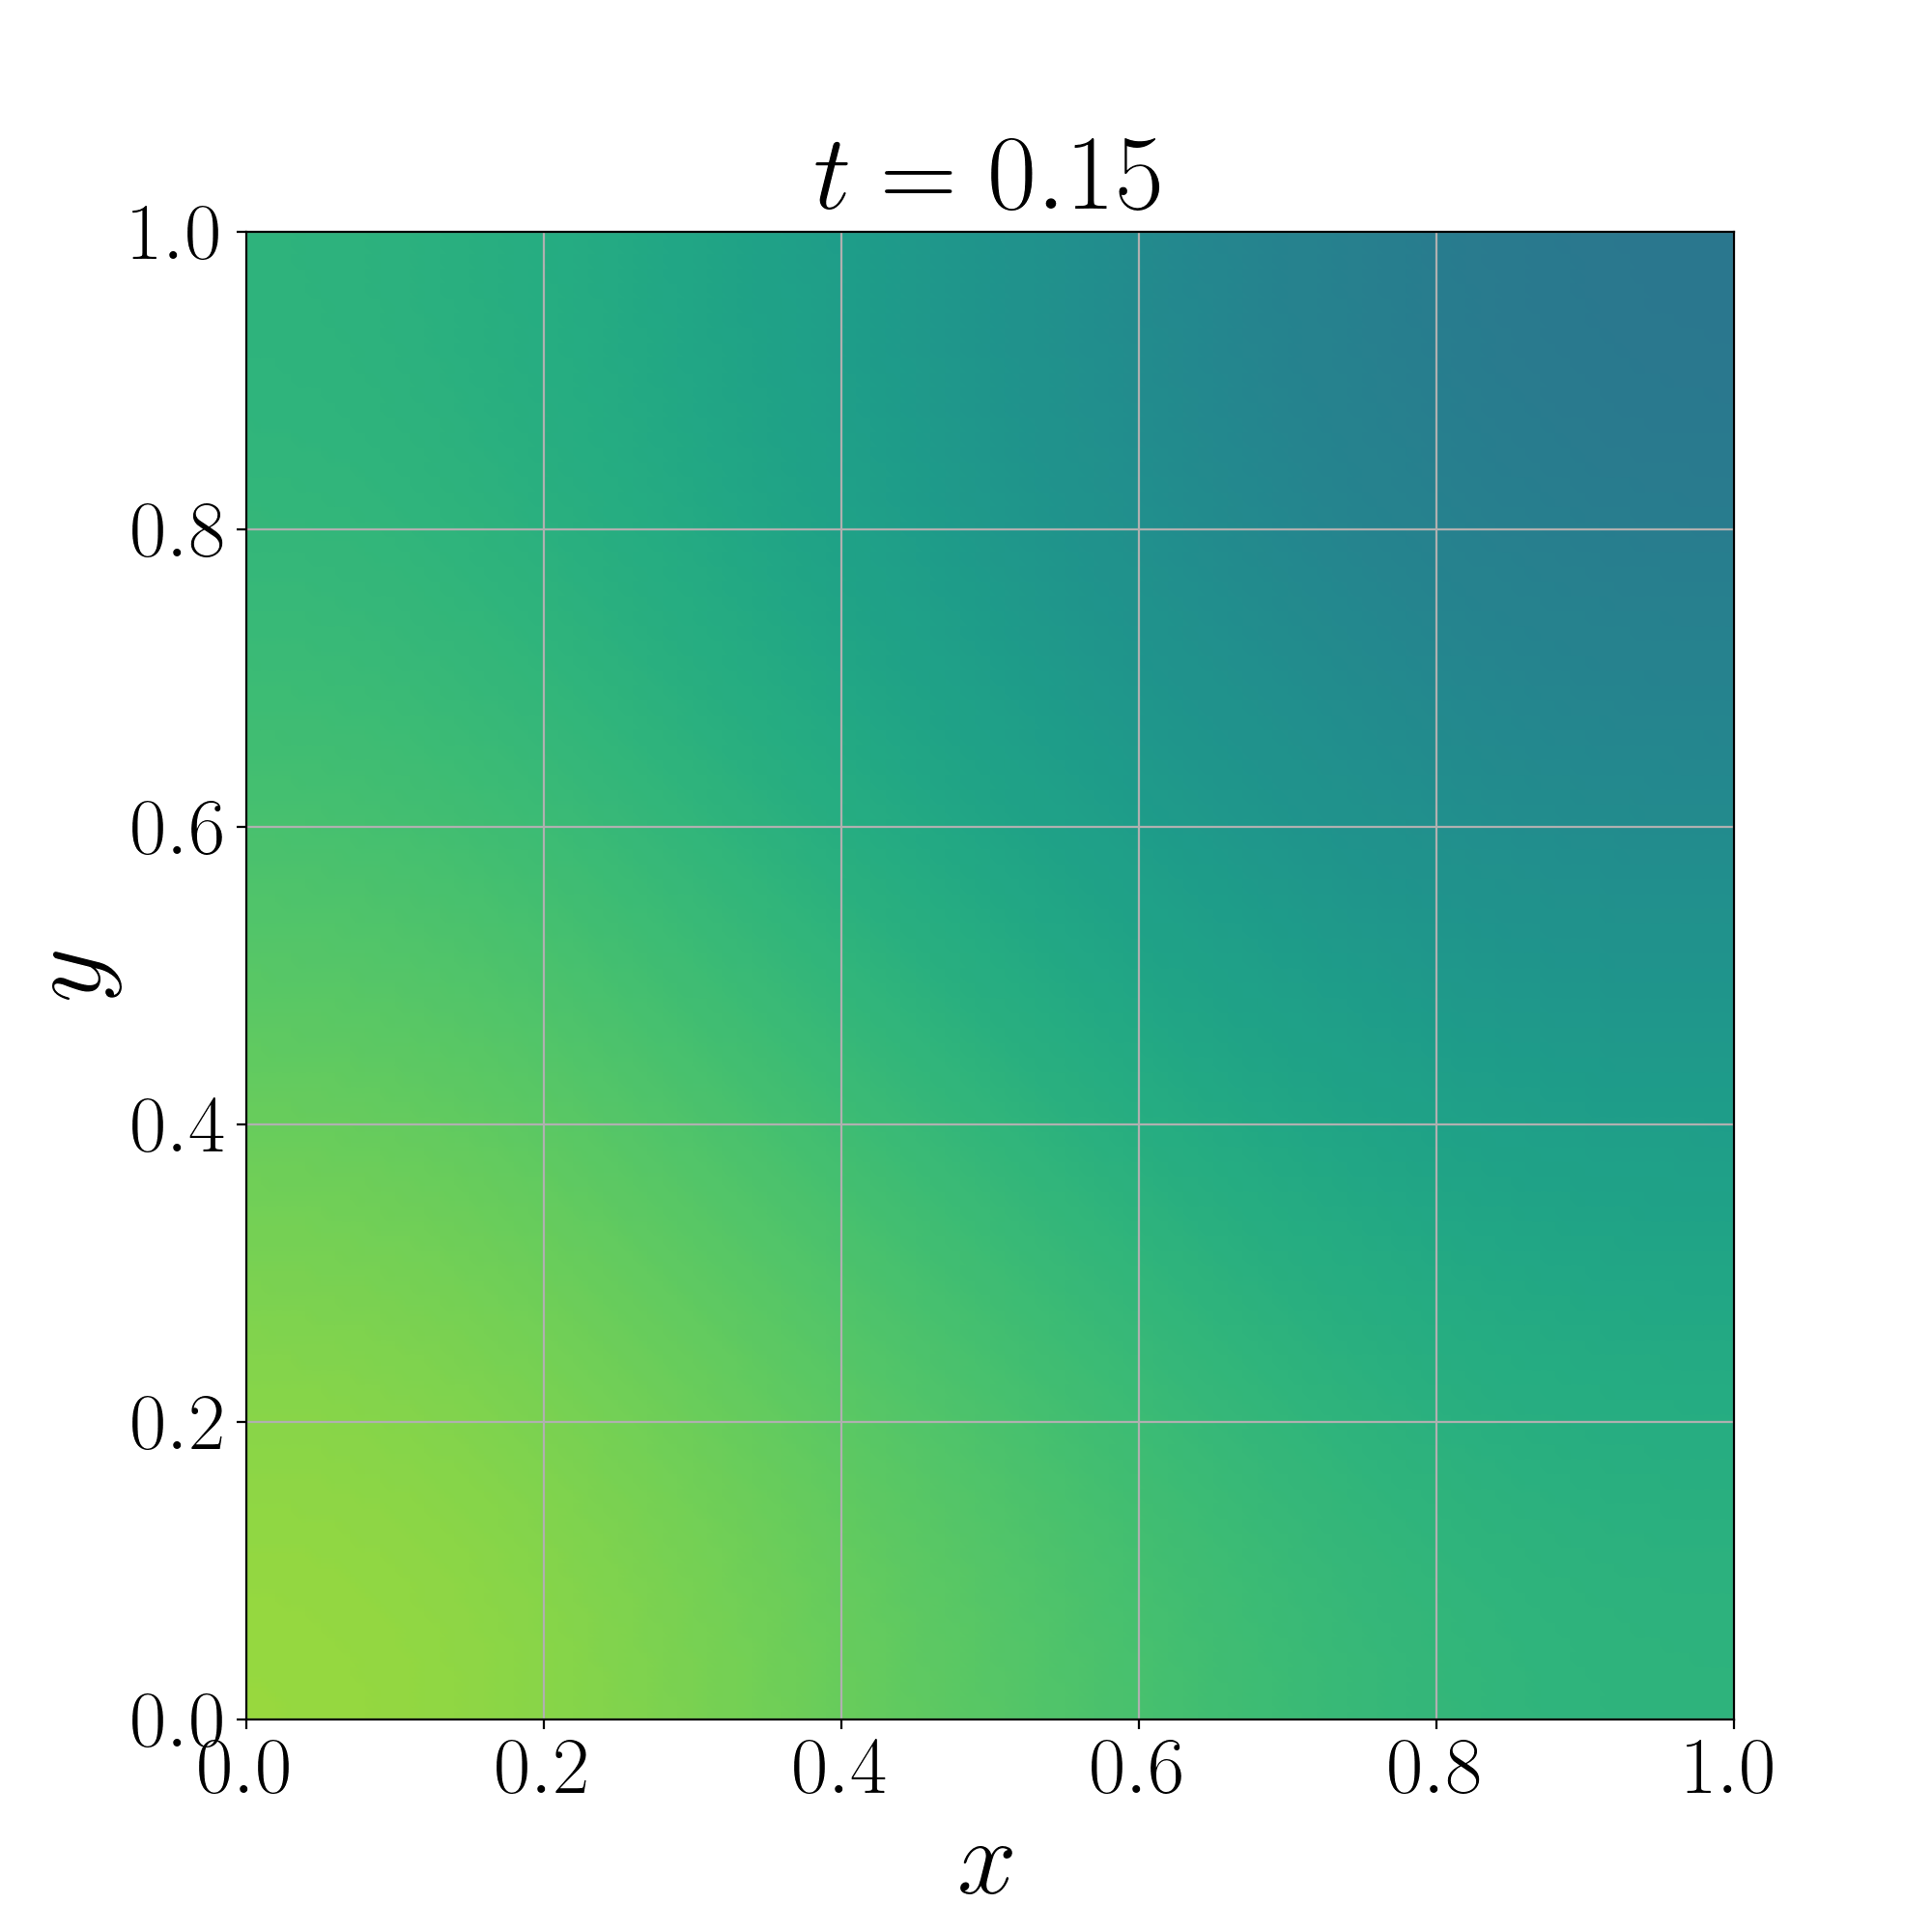
\includegraphics[width=\textwidth]{{./Input/cx_0p707_0p707_0p15}}};
\end{tikzpicture}
% =========================================================================================================
% =========================================================================================================
% t=0.5
\begin{tikzpicture}
\node[inner sep=0pt] (mixed) at (0,0)
{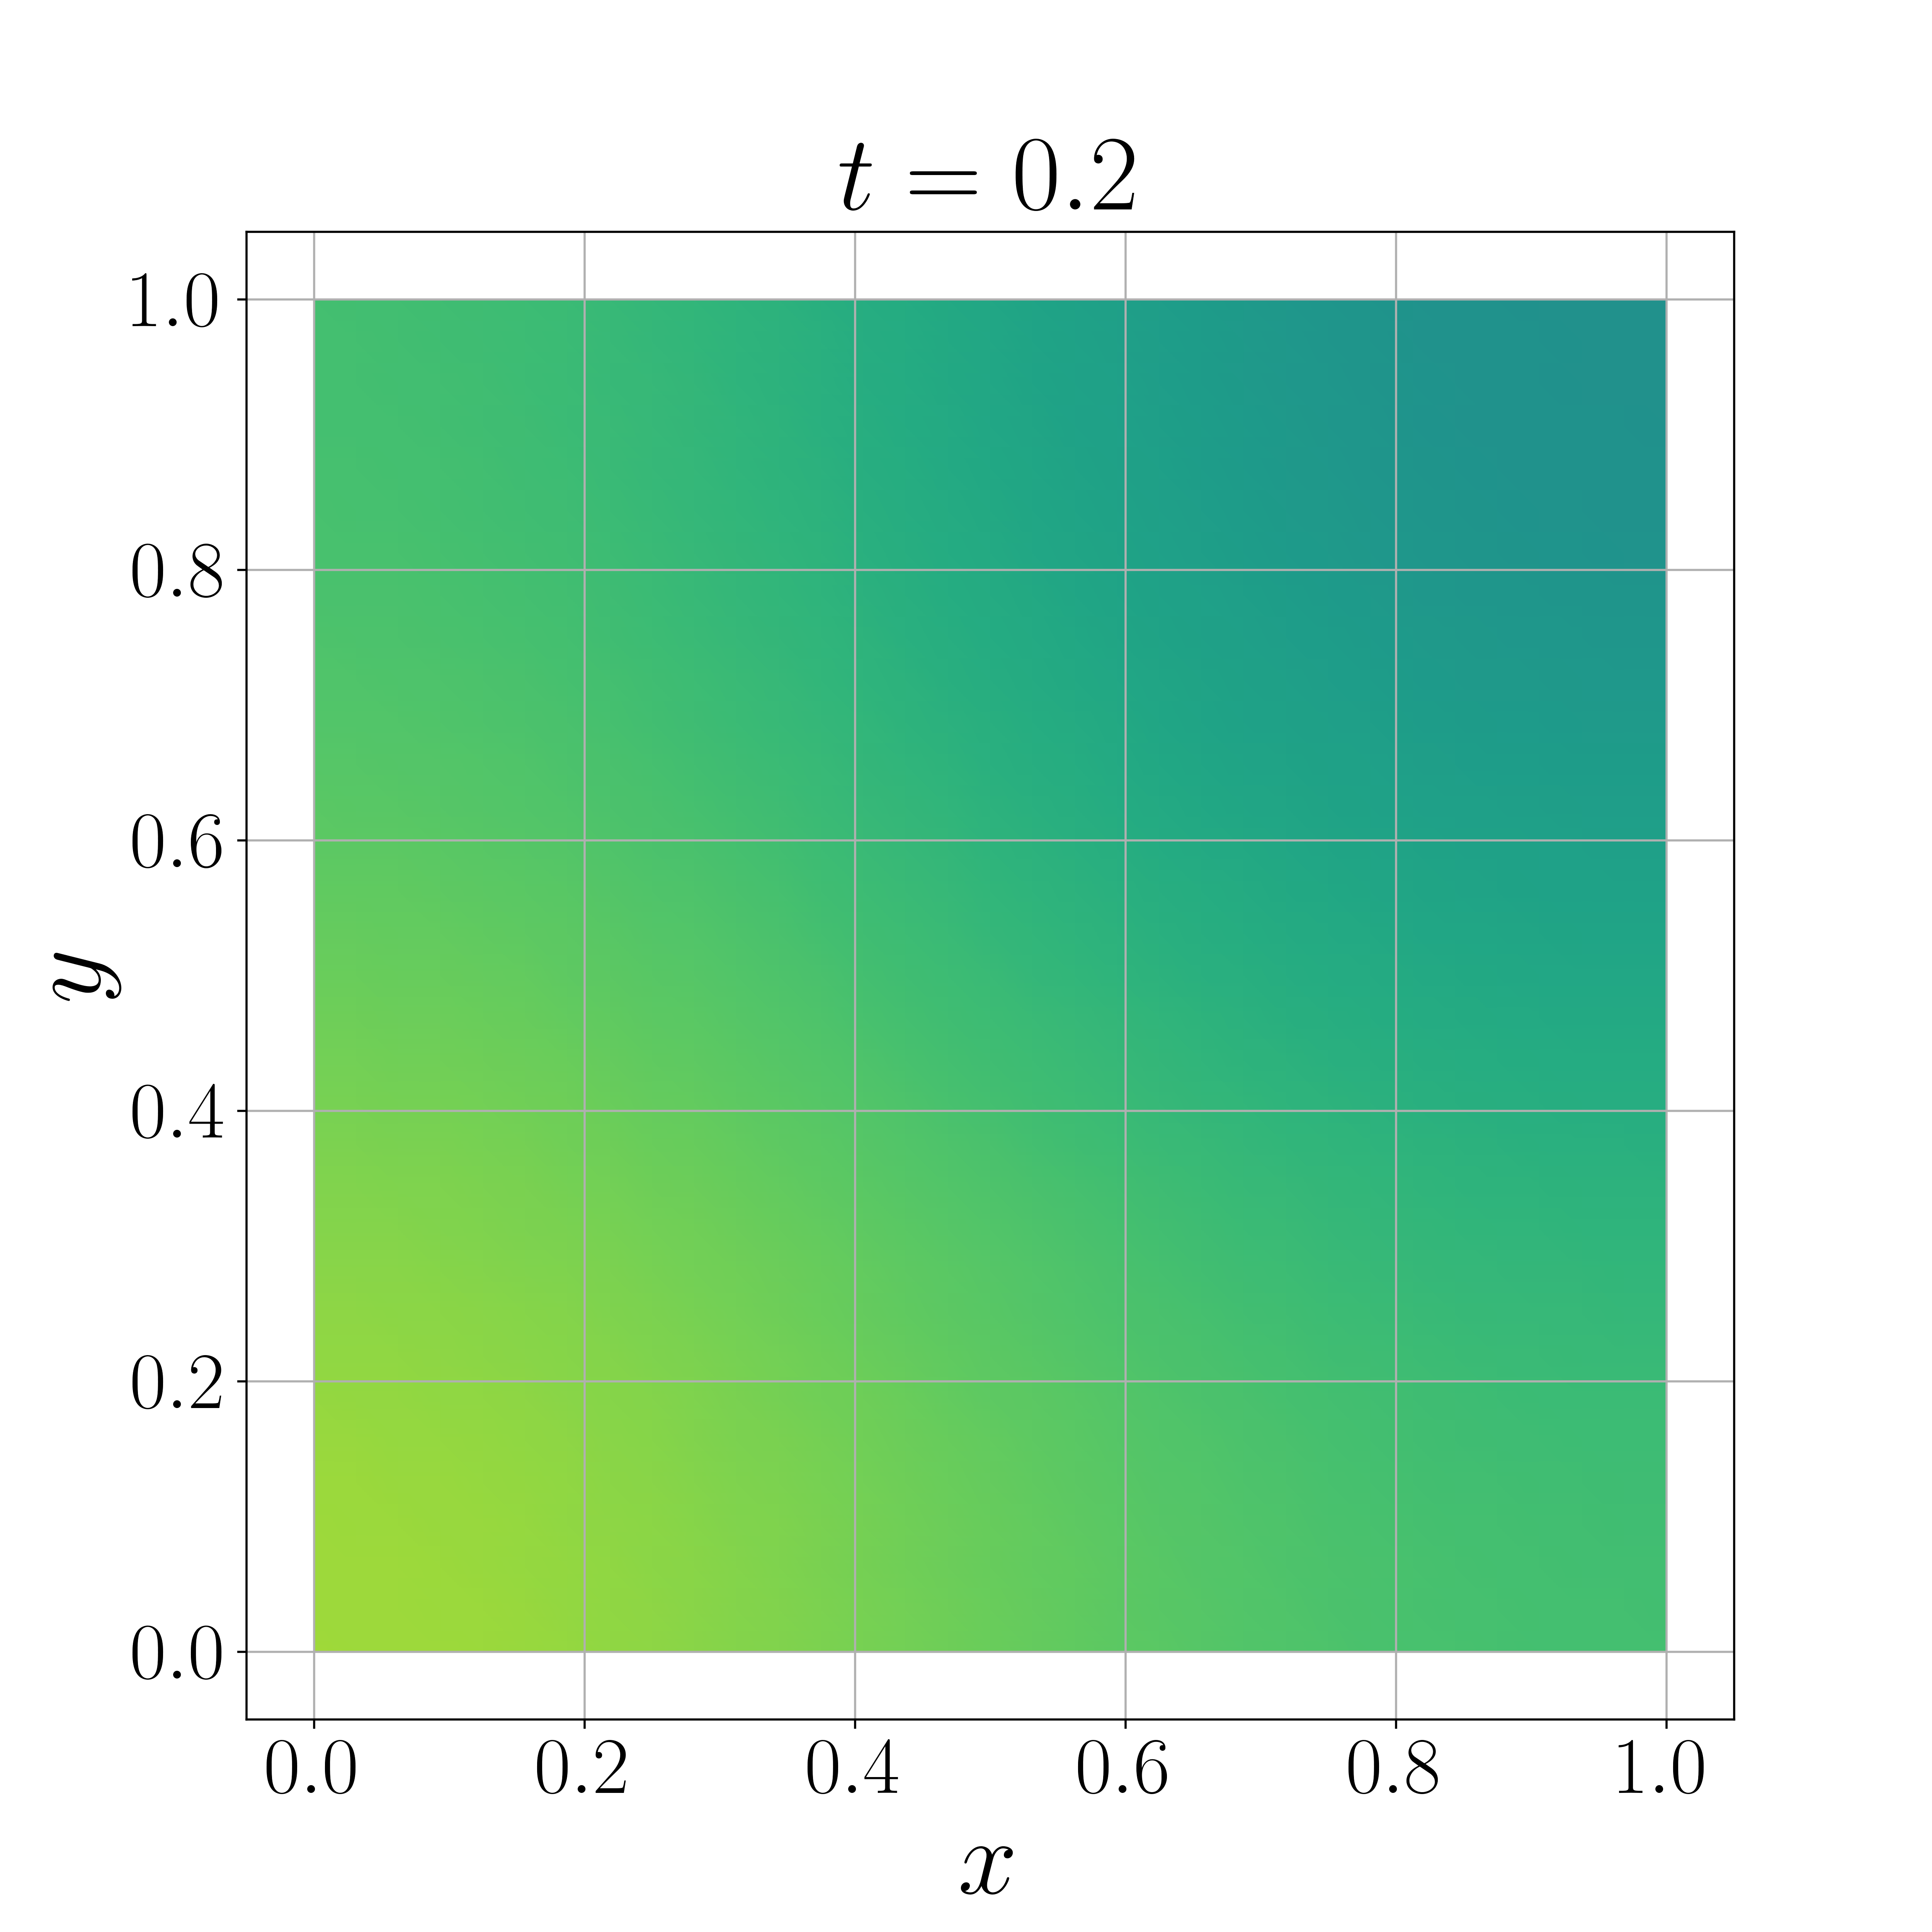
\includegraphics[width=\textwidth]{{./Input/cx_0p707_0p707_0p2}}};
\end{tikzpicture}
% =========================================================================================================
% =========================================================================================================
% t=0
\begin{tikzpicture}
\node[inner sep=0pt] (mixed) at (0,0)
{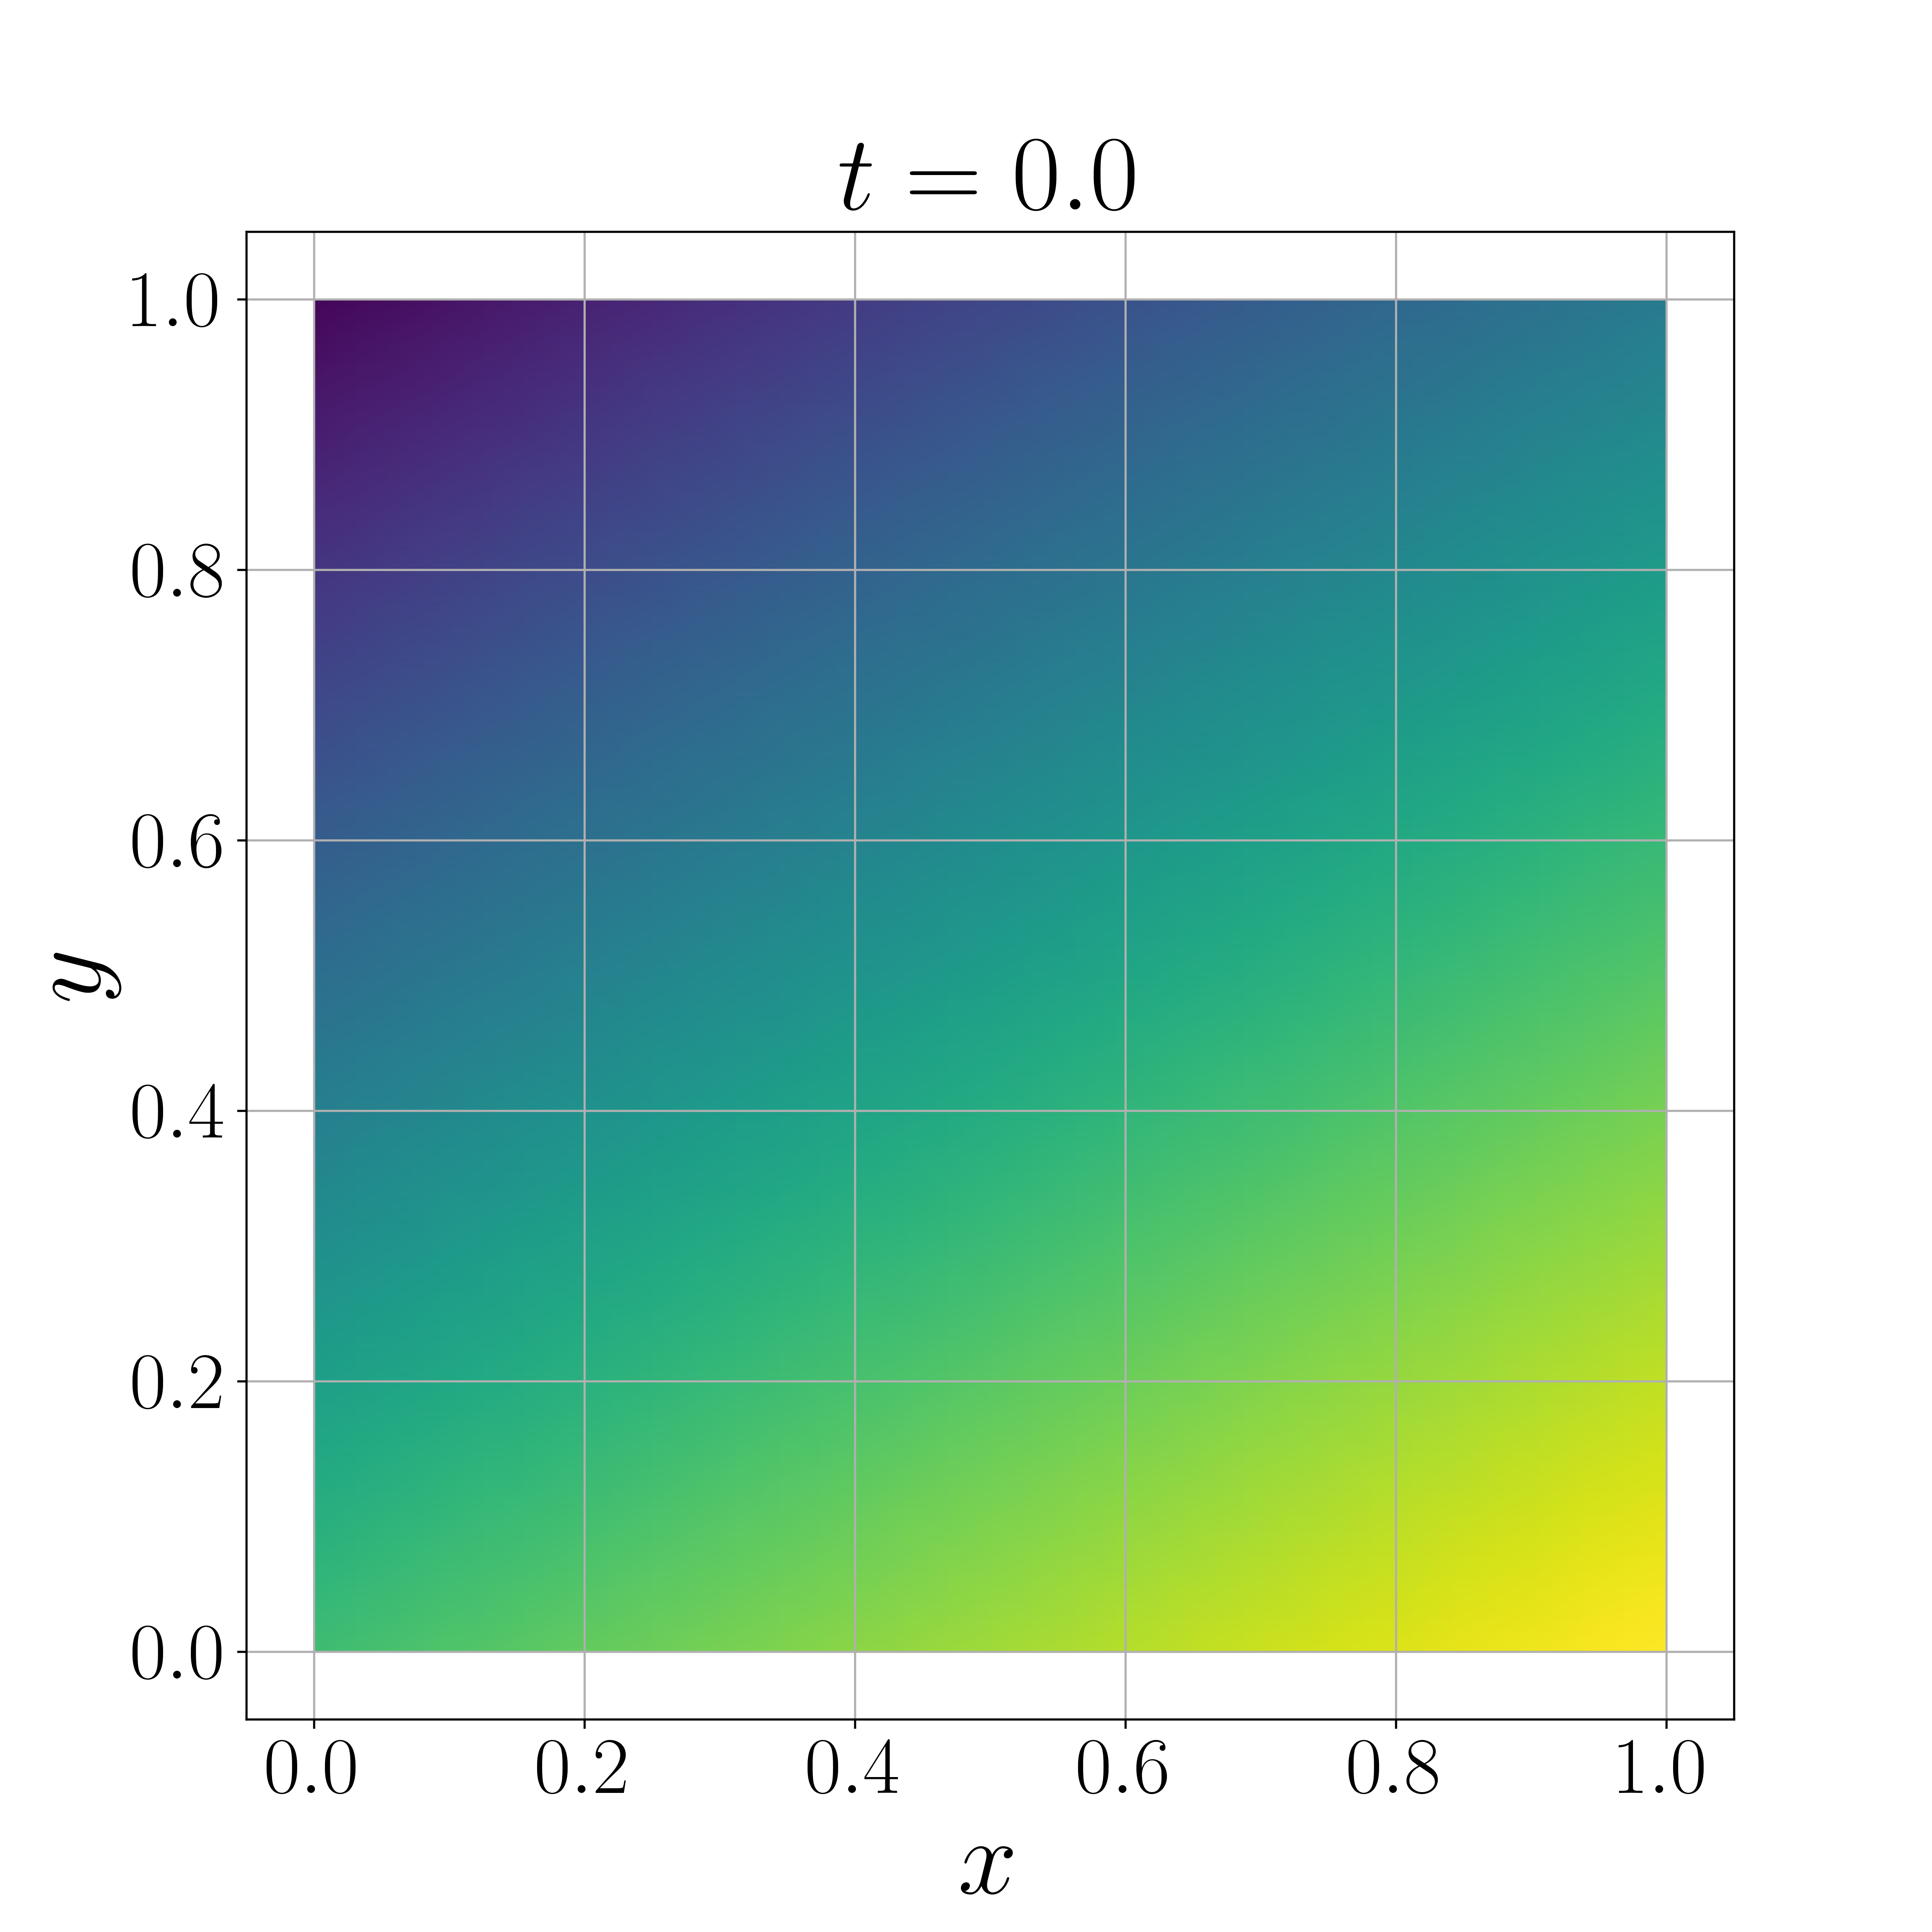
\includegraphics[width=\textwidth]{{./Input/cx_-0p5_0p866_0p0}}};
\end{tikzpicture}
% =========================================================================================================
% =========================================================================================================
% t=0.2
\begin{tikzpicture}
\node[inner sep=0pt] (mixed) at (0,0)
{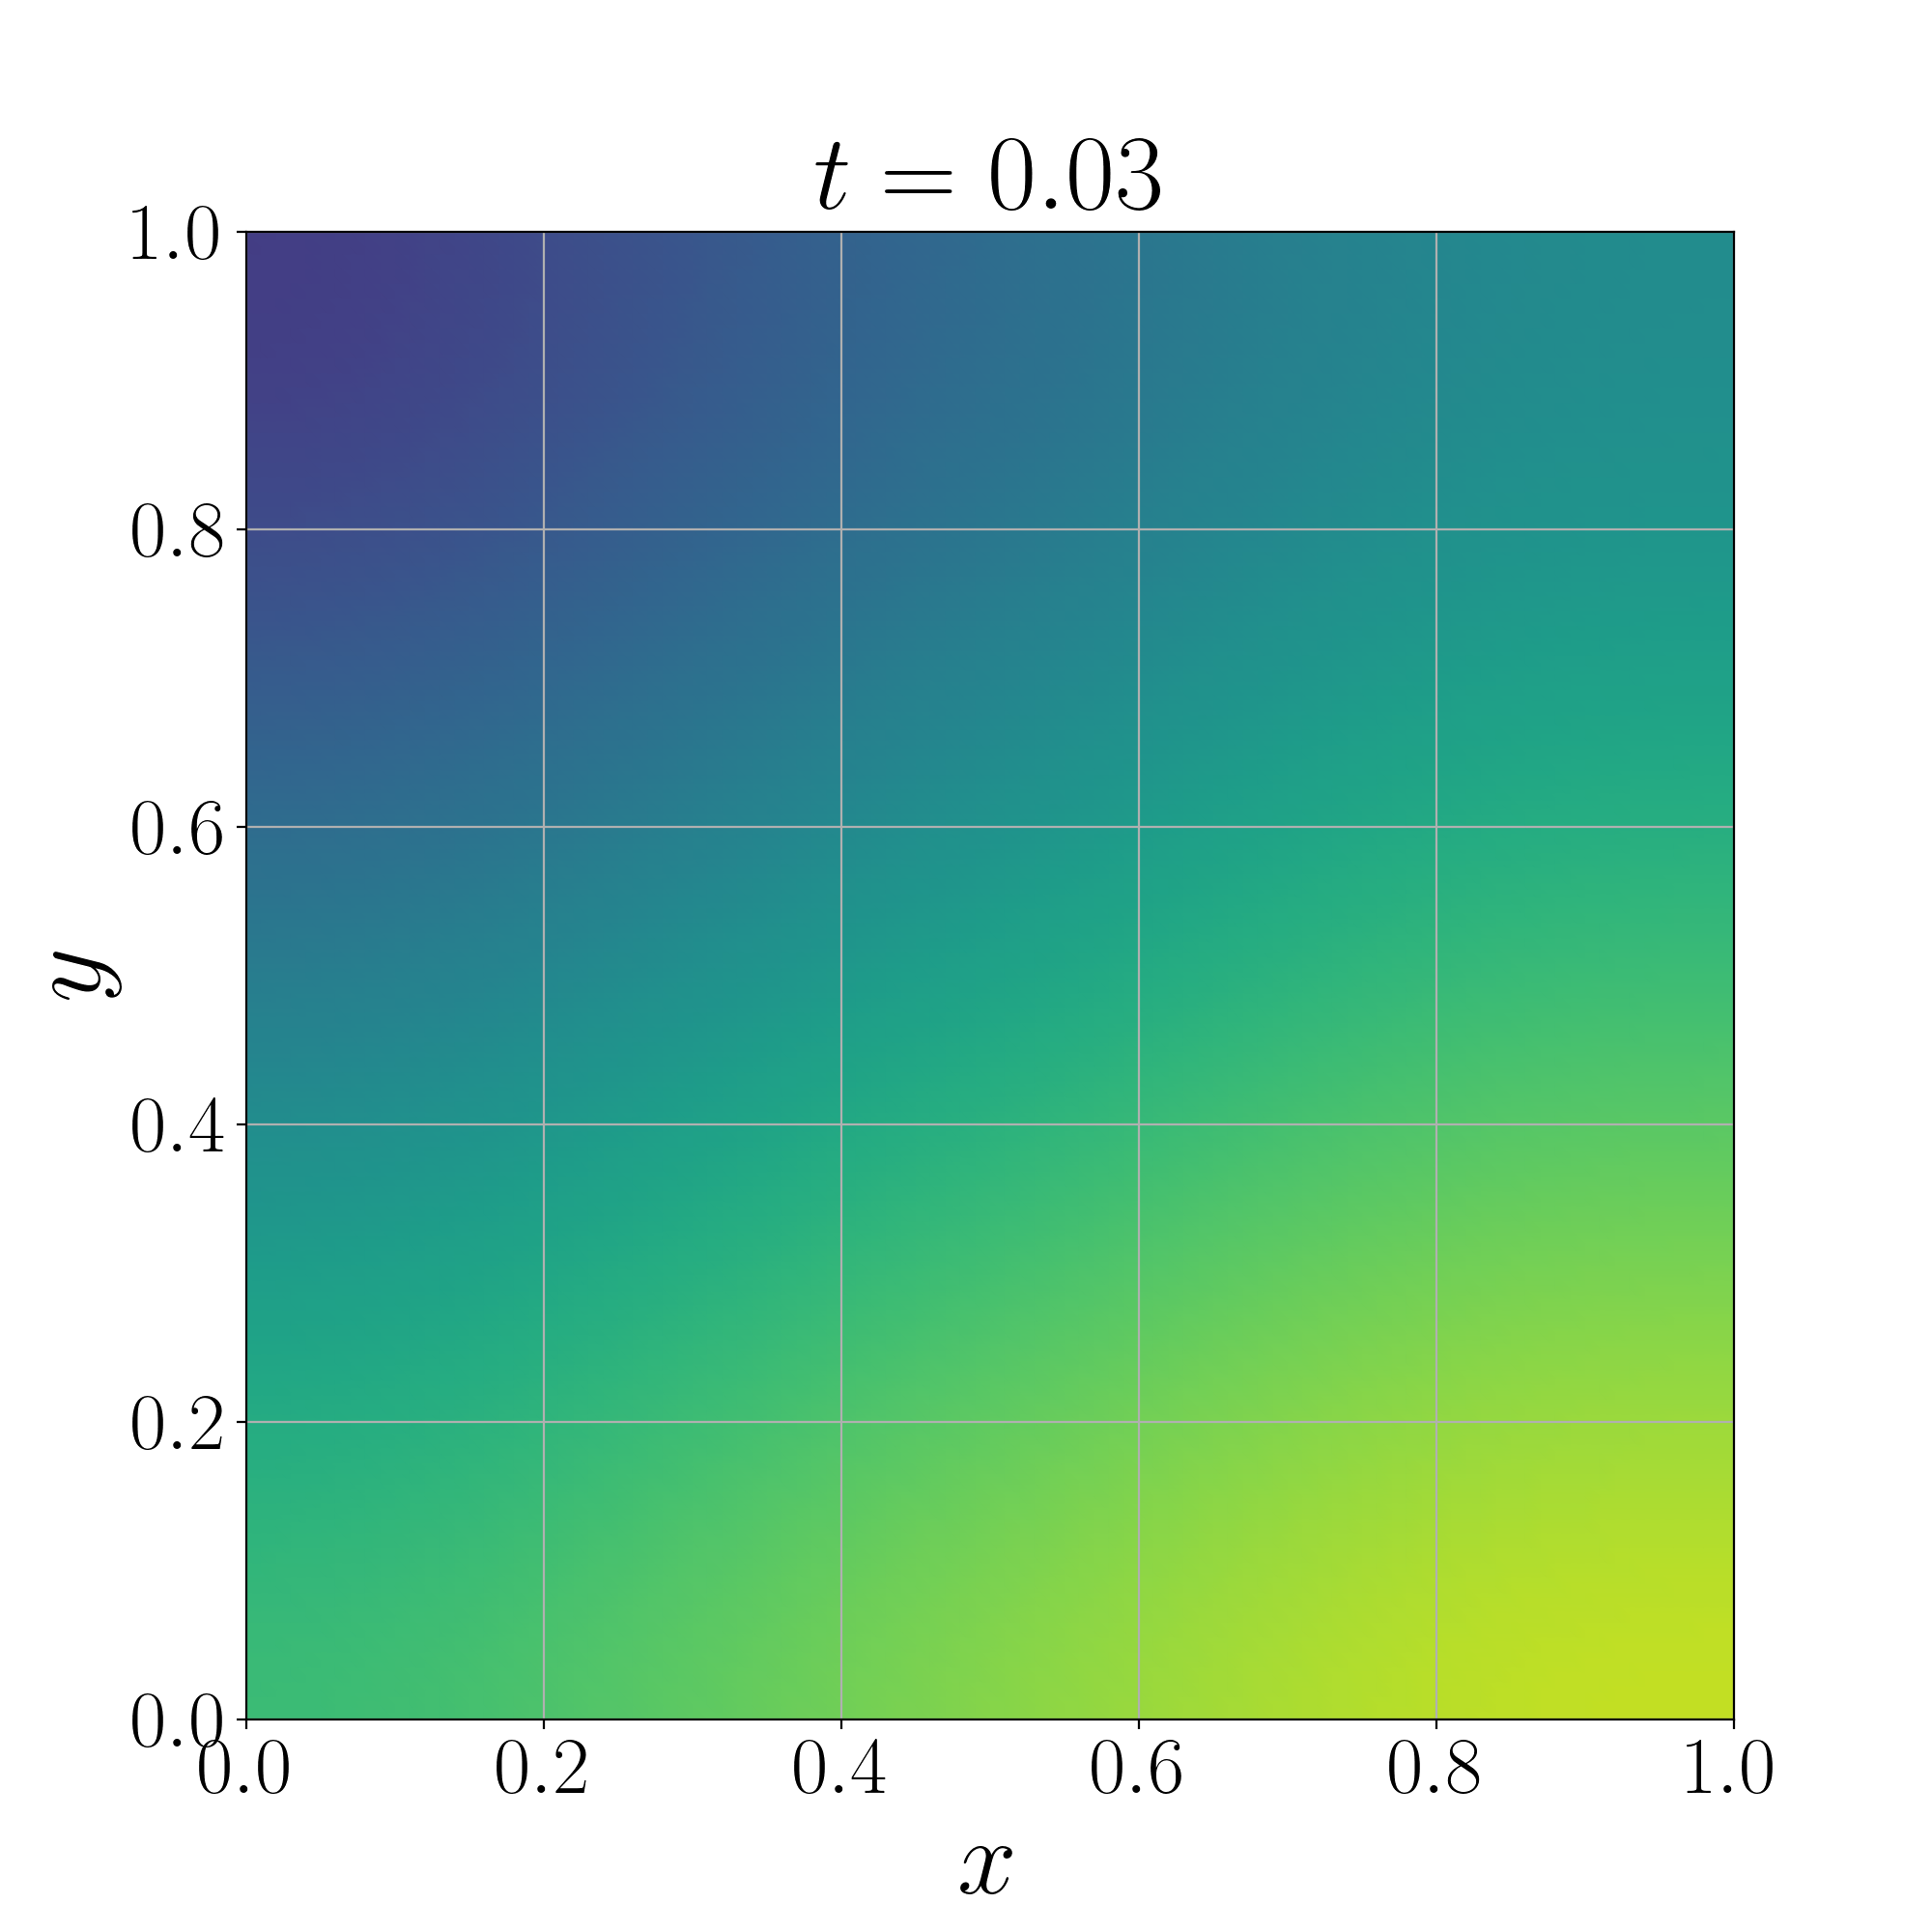
\includegraphics[width=\textwidth]{{./Input/cx_-0p5_0p866_0p03}}};
\end{tikzpicture}
% =========================================================================================================
% =========================================================================================================
% t=0.3
\begin{tikzpicture}
\node[inner sep=0pt] (mixed) at (0,0)
{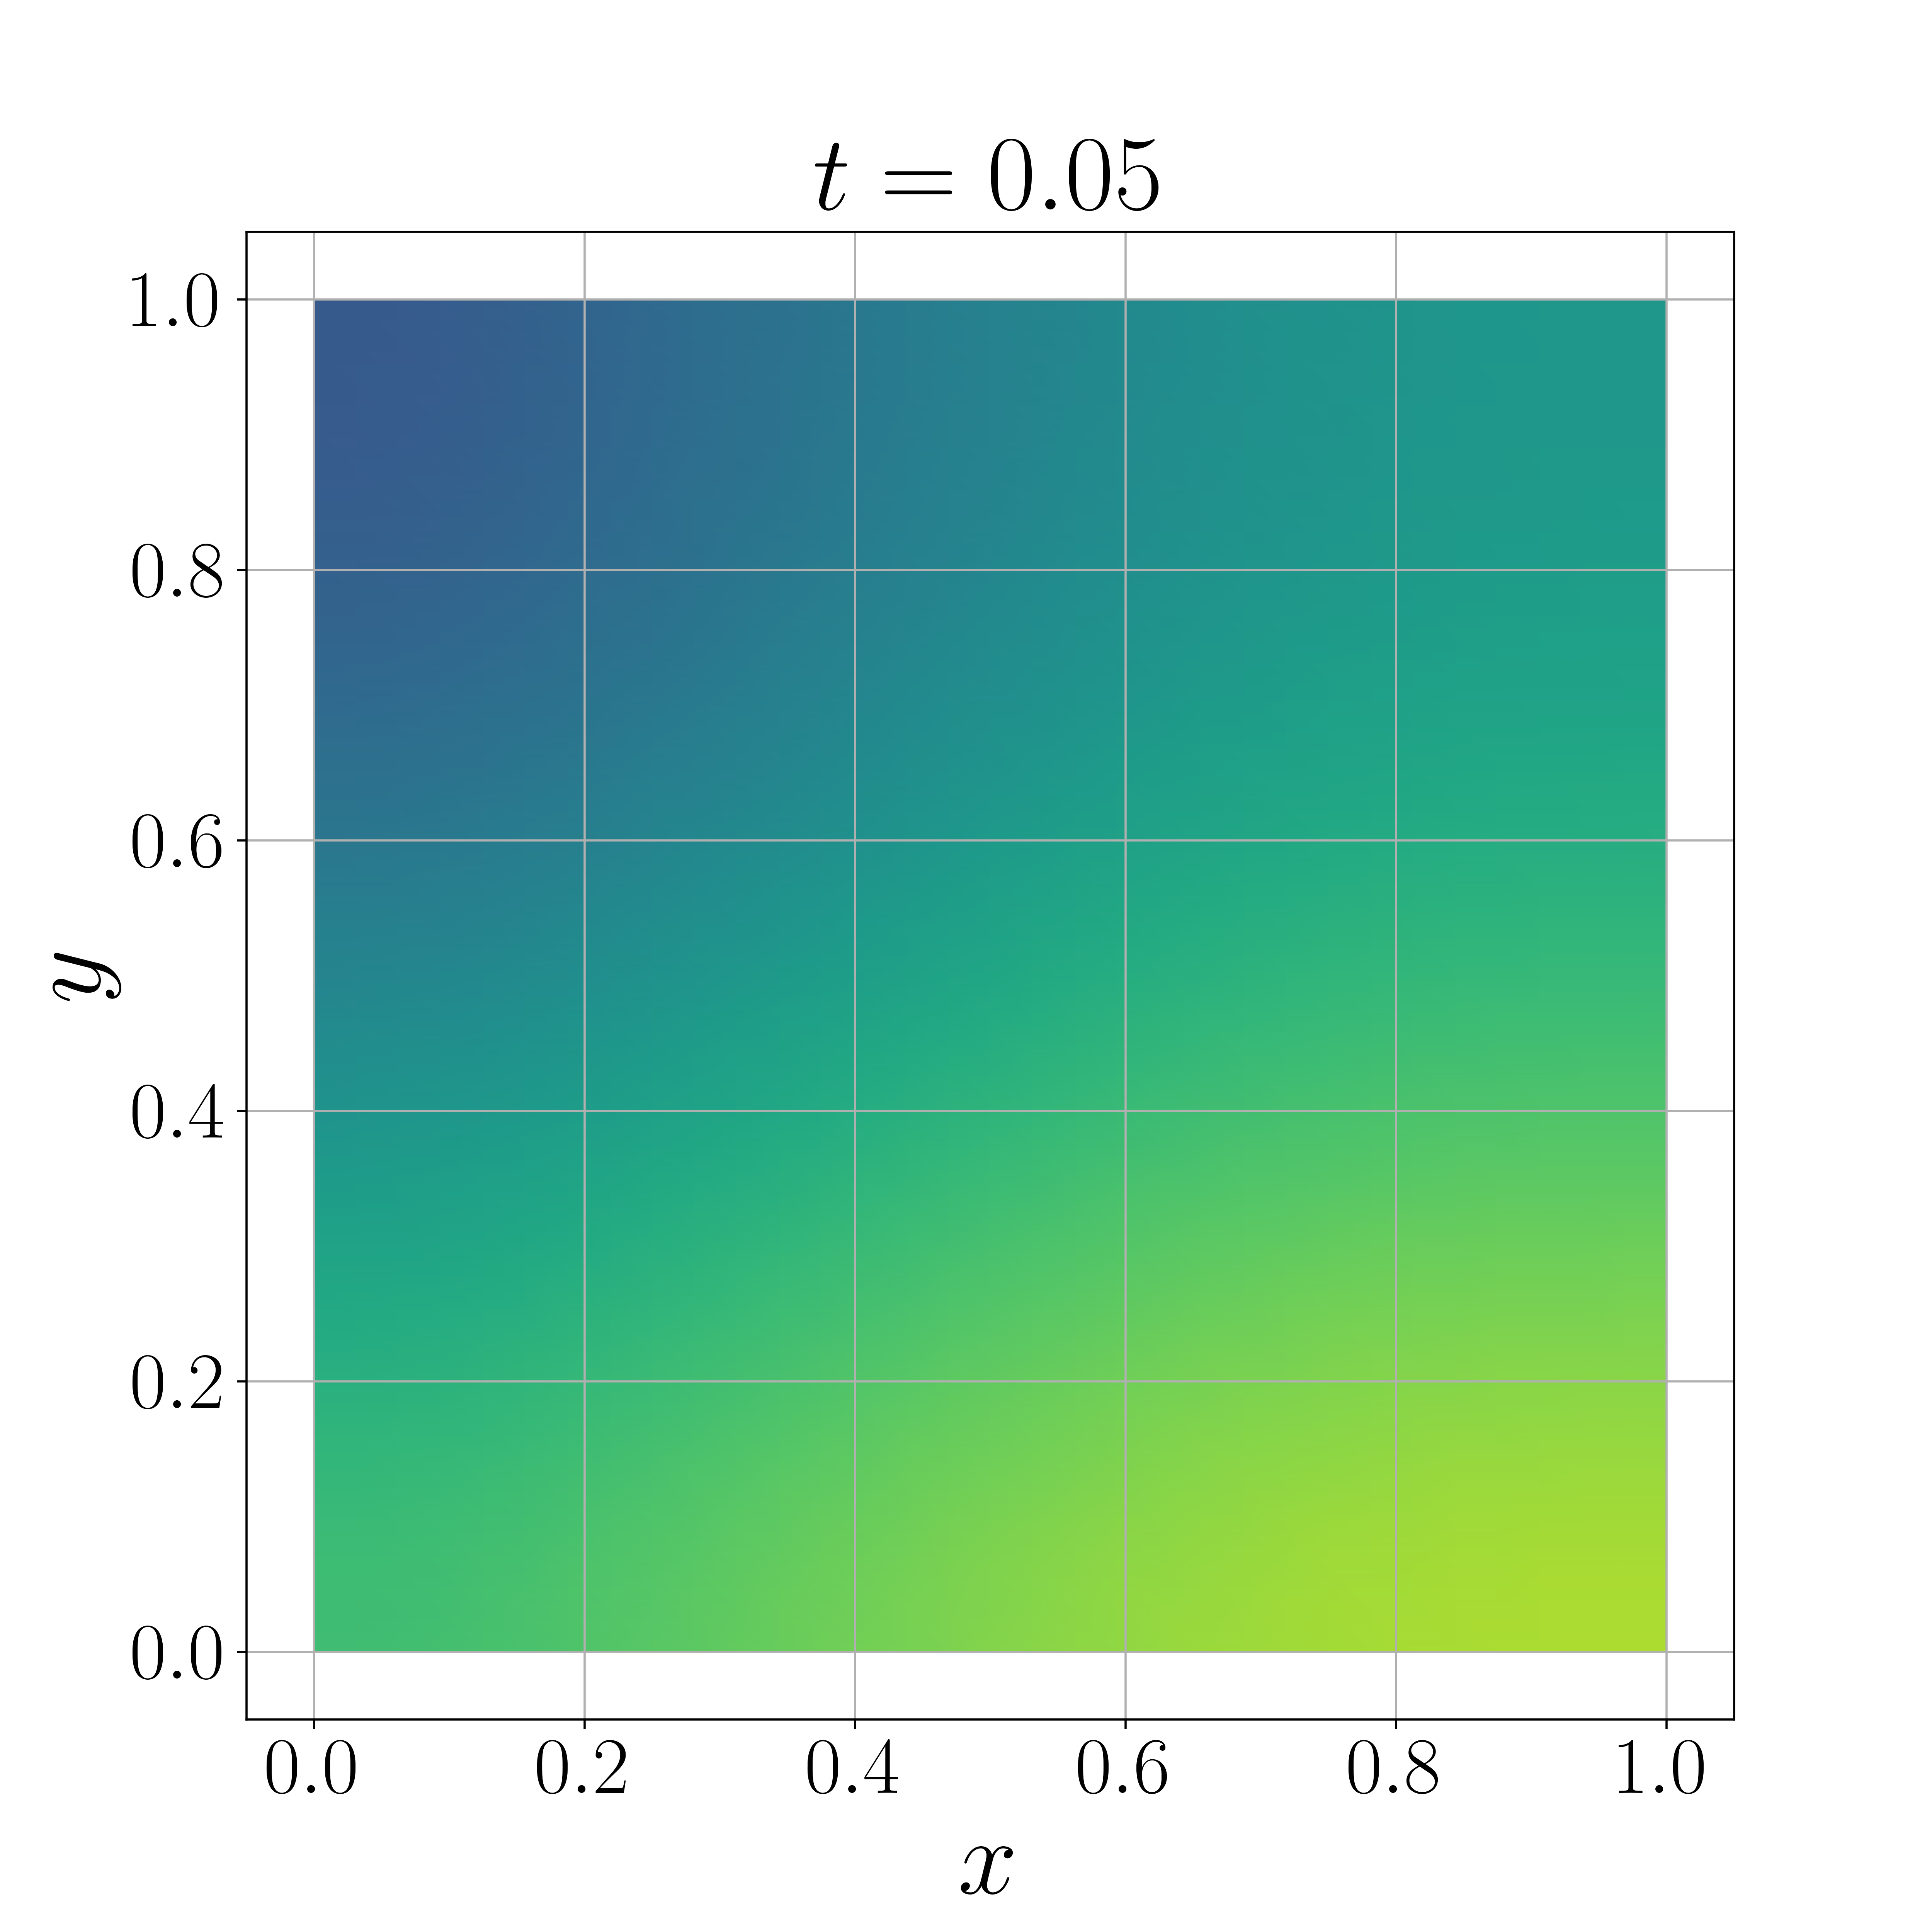
\includegraphics[width=\textwidth]{{./Input/cx_-0p5_0p866_0p05}}};
\end{tikzpicture}
% =========================================================================================================
% =========================================================================================================
% t=0.4
\begin{tikzpicture}
\node[inner sep=0pt] (mixed) at (0,0)
{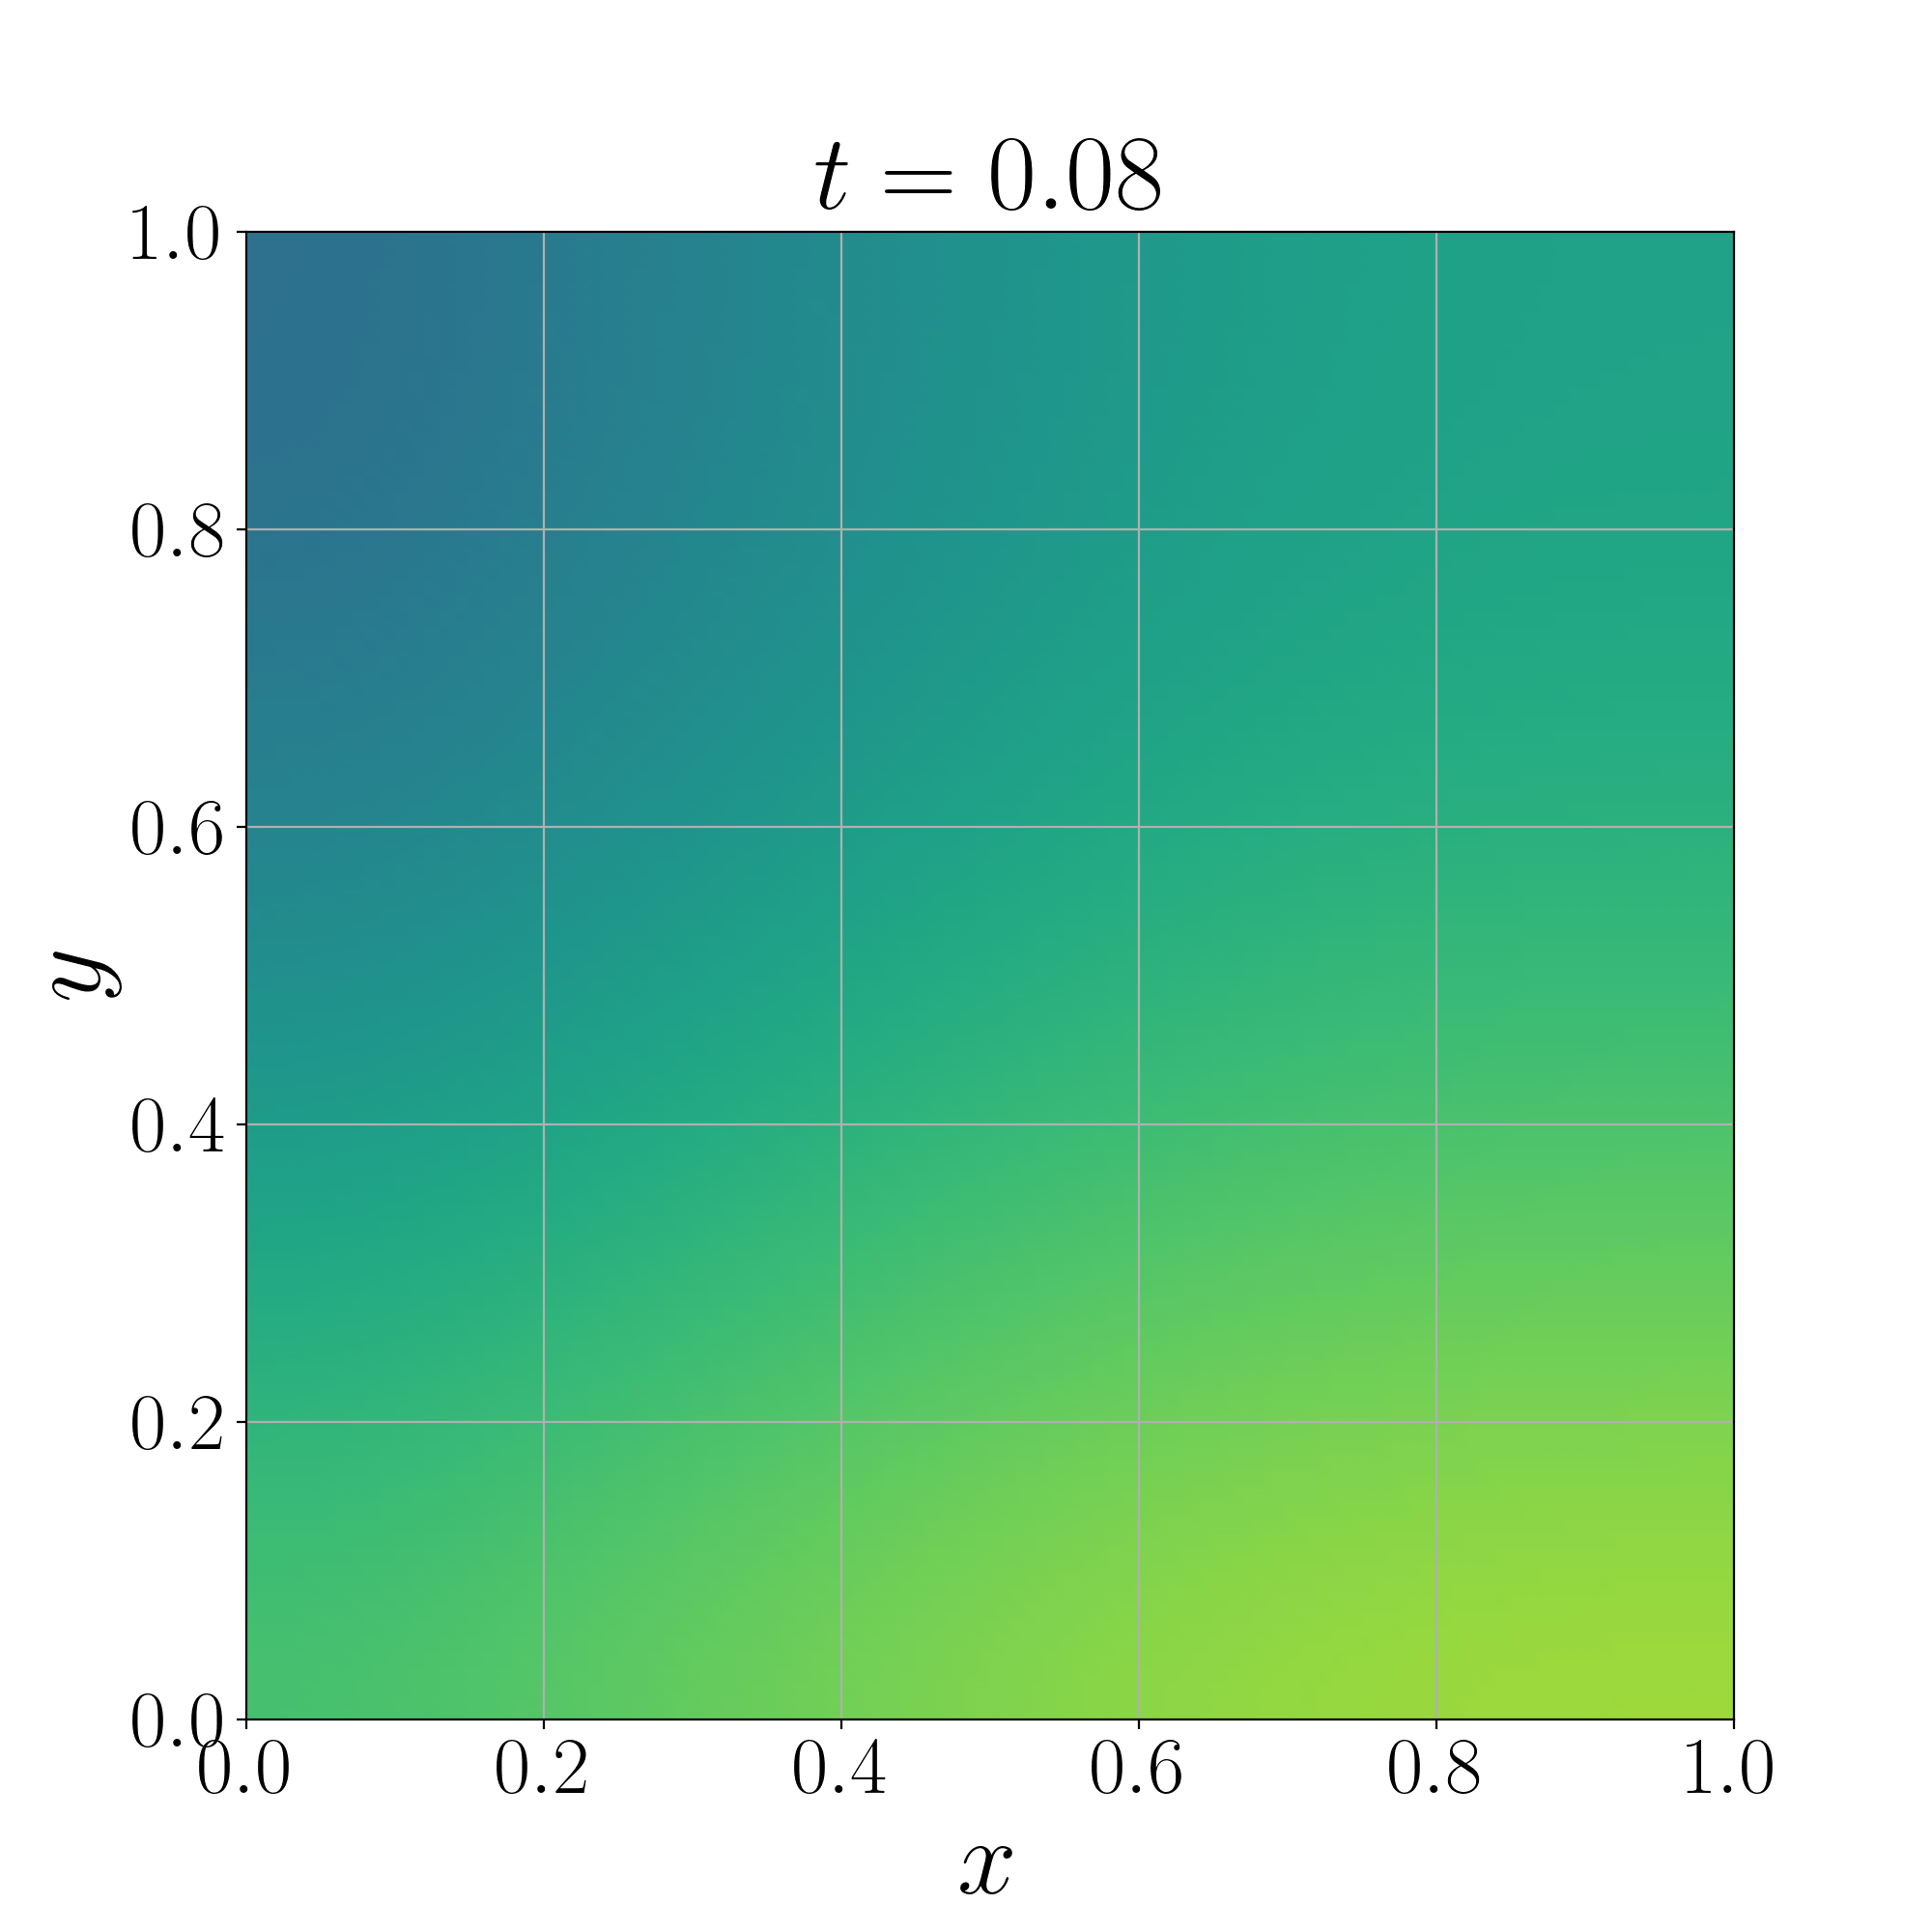
\includegraphics[width=\textwidth]{{./Input/cx_-0p5_0p866_0p08}}};
\end{tikzpicture}
% =========================================================================================================
% =========================================================================================================
% t=0.5
\begin{tikzpicture}
\node[inner sep=0pt] (mixed) at (0,0)
{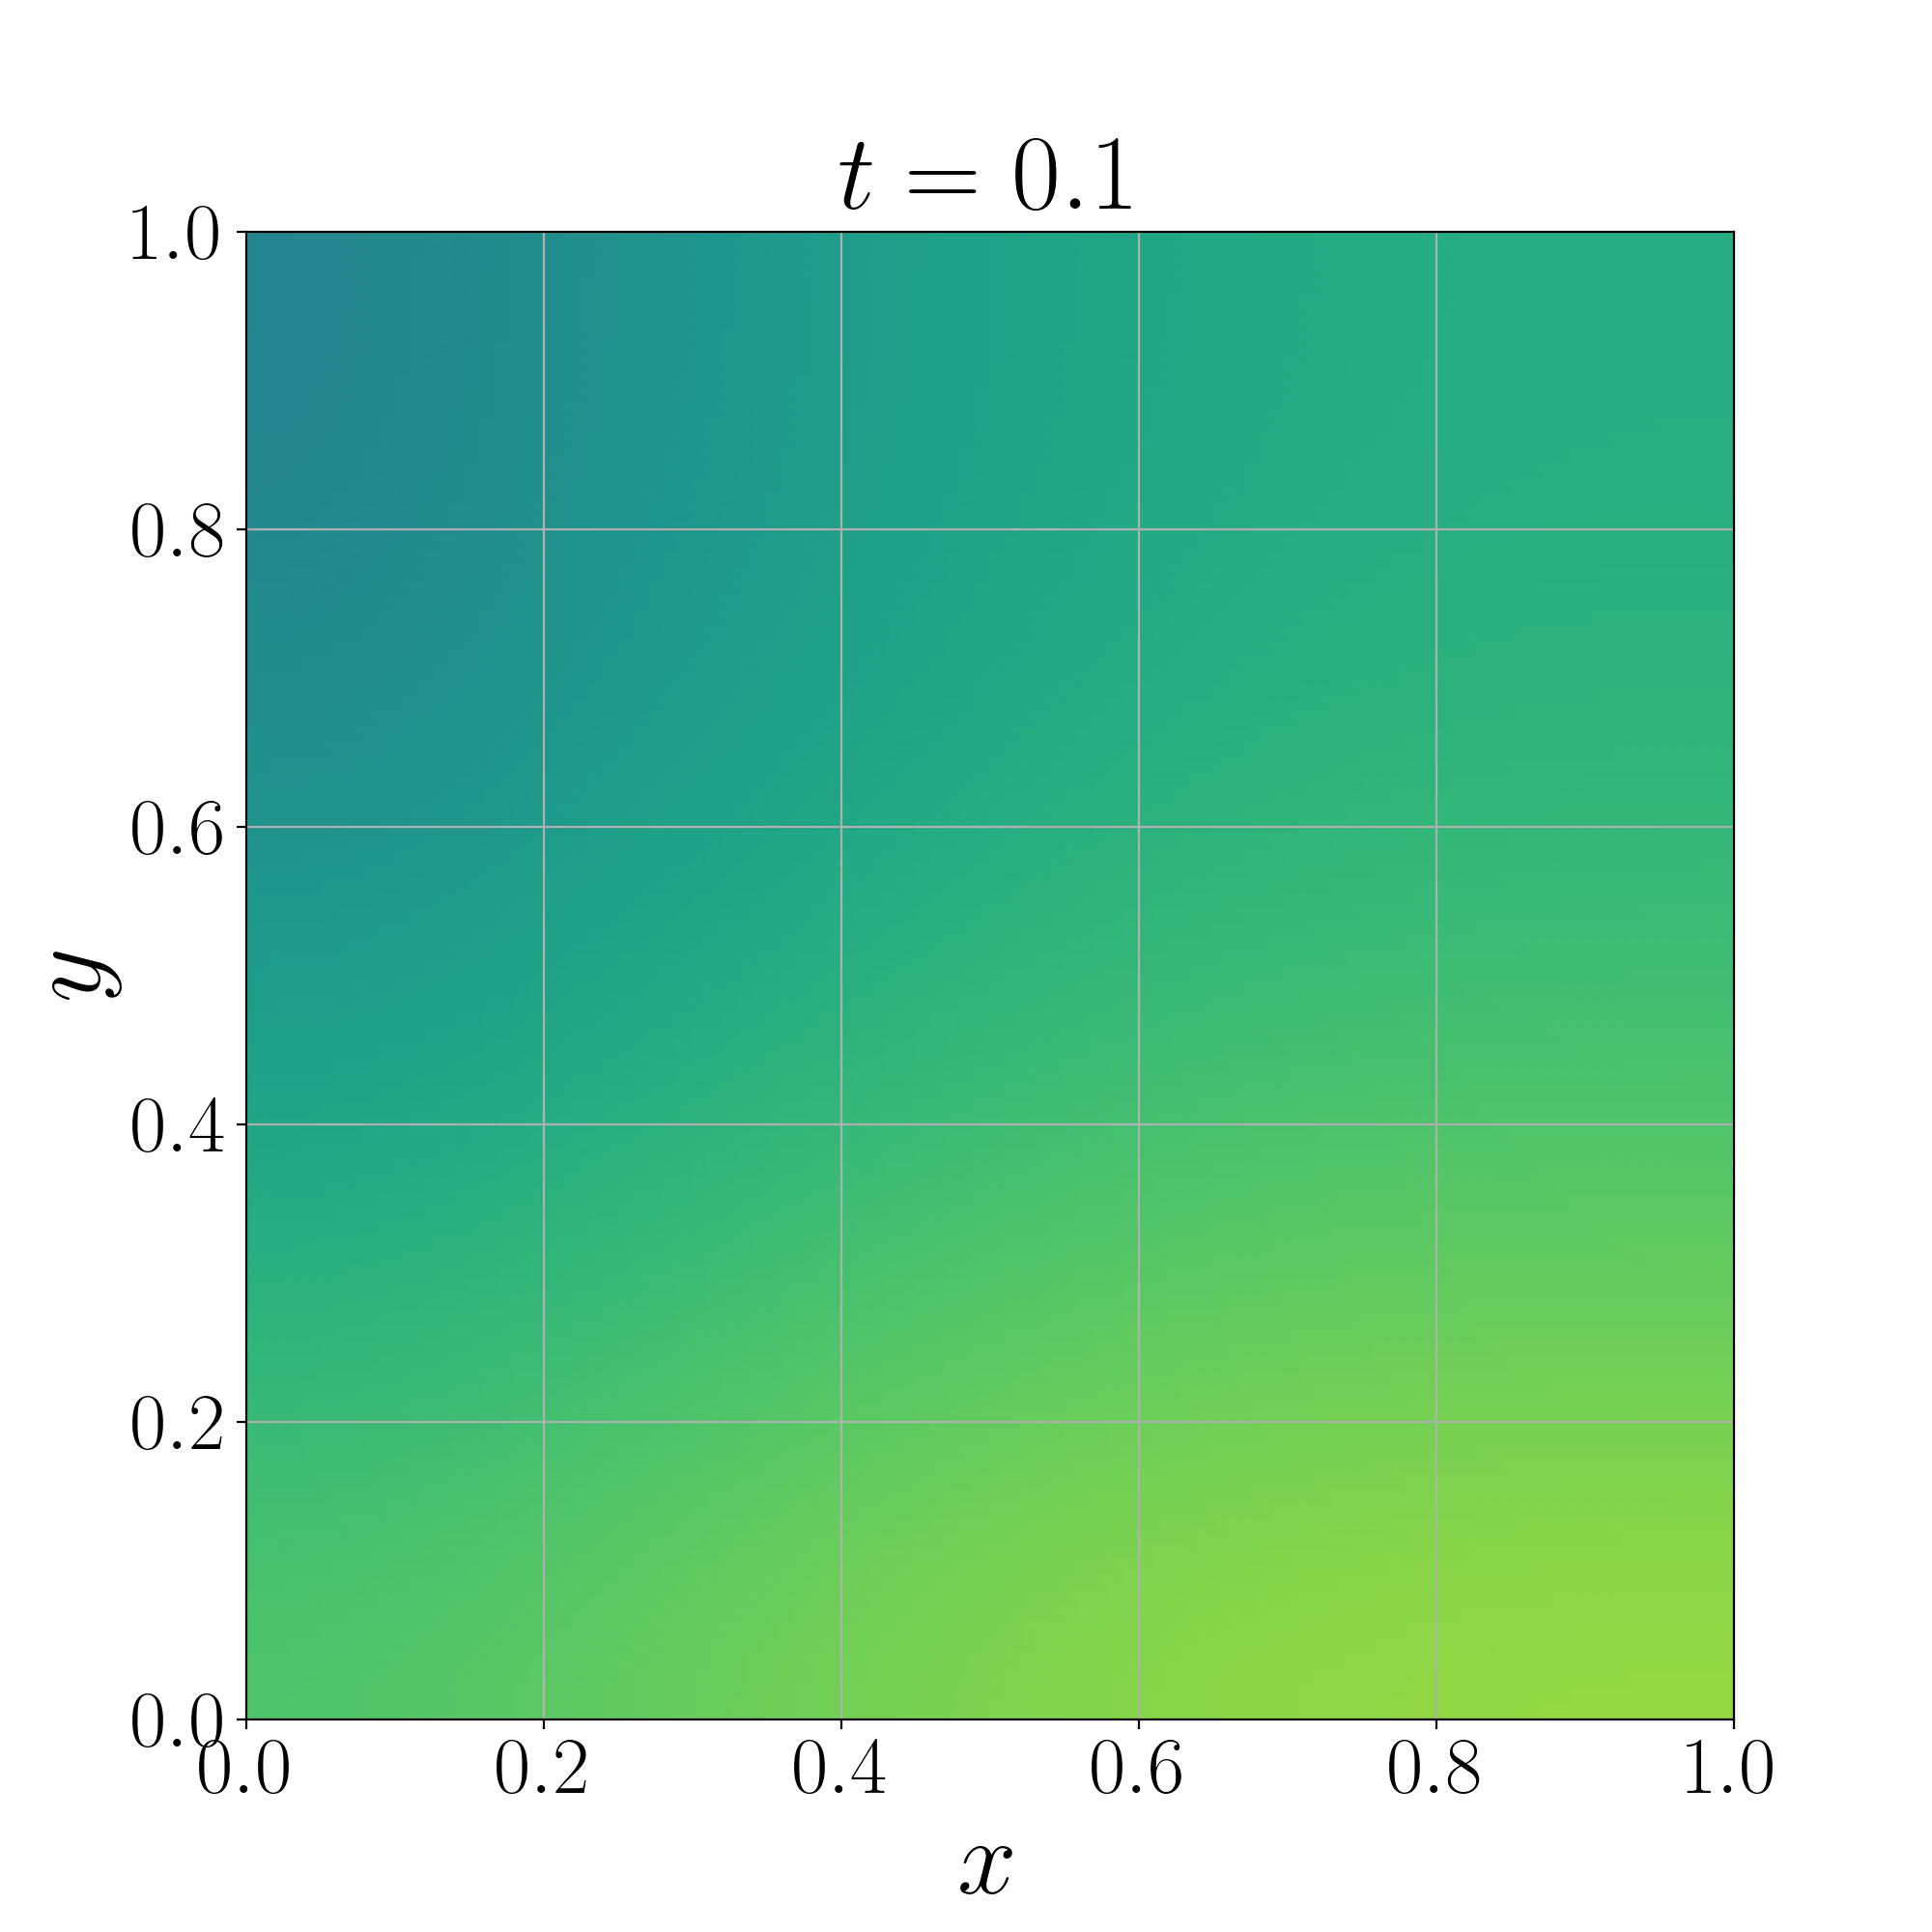
\includegraphics[width=\textwidth]{{./Input/cx_-0p5_0p866_0p1}}};
\end{tikzpicture}
% =========================================================================================================
\end{document}
